\chapter{2020 Progress Review}
\label{ch:progressreview2020}

\section{Introduction}\label{introduction}
By 2050 the world’s population is expected to increase to over 9 billion~\autocite{gerlandWorldPopulationStabilization2014}. Food production globally must increase by over \SI{100}{\percent} by 2050 to feed the growing population if current diets are unchanged~\autocite{tilmanGlobalFoodDemand2011,berners-leeCurrentGlobalFood2018}. Demand for non\hyp{}food plant crops such as those used as fermentation feedstocks for biofuels and industrial microbial manufacturing, and plants producing therapeutic compounds is also likely to increase. Since the Green Revolution, where crop yields were dramatically increased through plant breeding, plant breeders have failed to increase food production to match population growth~\autocite{kropffQuantitativeUnderstandingYield1994,zhuImprovingPhotosyntheticEfficiency2010}. Genetic variation within coding sequences has been heavily exploited for crop improvement. For example, markers identified in coding sequences by transcriptome or exome resequencing can be used in marker assisted breeding~\autocite{varshneyGeneBasedMarkerSystems2009}. However, quantitative, complex traits that respond to changes in the environment are the result of genetic and epigenetic variation in the non\hyp{}coding regulatory sequences of multiple genes. Plant growth in response to environmental change is coordinated by suites of genes working combinatorially within complex gene regulatory networks (GRNs). These GRNs are composed of many connections, including those between transcription factors (TFs) and recognition sequences in the genes they regulate. By applying synthetic biology approaches, researchers working in microorganisms have investigated the intrinsic properties of regulatory elements and used these rules to design new sequences with known properties~\autocite{curranDesignSyntheticYeast2014,zessConstructionNewSynthetic2016,rajkumarEngineeringSyntheticStressresponsive2016,machensSyntheticPromotersTranscription2017,cuperusDeepLearningRegulatory2017}. These approaches included modifying transcription factor binding sites (TFBSs) to create synthetic inducible promoters responding to certain stresses or to synthetic transcription factors. However, very few similar investigations of regulatory sequences in the genomes of multicellular eukaryotes, including plants, have been done. A greater understanding of the functional components of plant regulatory sequences would enable the design of synthetic regulatory sequences (DNA parts) that can be used to engineer plants to perform new functions. It would also enable the identification of useful mutations in breeding populations and inform the engineering or editing of endogenous regulatory sequences for crop improvement.

\subsection{Regulation of gene
expression}\label{regulation-of-gene-expression}
The expression of genes is regulated at several points including transcription, mRNA stability and processing, gene silencing and translation. Transcription is the first level of control and, for many protein\hyp{}coding genes, the rate of transcription will strongly influence
the abundance of the encoded protein~\autocite{liuDependencyCellularProtein2016}. Transcription is controlled by the interactions of certain proteins with DNA regulatory sequences resulting in increases or decreases in gene expression. In eukaryotes, there are two types of DNA regulatory sequences called \textit{cis}\hyp{}regulatory and \textit{trans}\hyp{}regulatory sequences.


\subsubsection{\texorpdfstring{\textit{Cis}-regulatory DNA
sequences}{Cis\hyp{}regulatory DNA sequences}}\label{cis-regulatory-dna-sequences}
\textit{Cis}\hyp{}regulatory sequences are those on the same molecule of DNA as the gene they regulate. The literature varies when defining \textit{cis}\hyp{}regulatory sequences. For example, \textcite*{wittkoppCisregulatoryElementsMolecular2012} broadly define both promoters and enhancers as \textit{cis}\hyp{}regulatory elements (CREs). This report, in line with \textcite*{swinnenLessonsDomesticationTargeting2016}, defines CREs as small individual motifs within regulatory sequences which can bind to the DNA binding domain of one or more \textit{trans}\hyp{}acting molecules such as transcription factors and non\hyp{}coding RNAs (ncRNAs). Therefore, both transcription factor binding sites (TFBS) and ncRNA binding sites (such as triplex targeting sites) are types of CREs.
A \textit{cis}\hyp{}regulatory module (CRM) is defined as a genomic region encompassing multiple CREs that together regulate an aspect of gene expression pattern~\autocite{guoNewAlgorithmIdentifying2017}. CRMs may include promoters, enhancers, silencers, insulators and locus control regions~\autocite{jeziorskaSystemsBiologyApproach2009}. CRMs can be located within exons~\autocite{tumpelRegulatoryModuleEmbedded2008}, introns~\autocite{ostrovskyIdentificationStrongIntron2018}, 5’\hyp{}untranslated regions (5’UTRs)~\autocite{bolleSegmentsEncodingUntranslated1994,henrySharedCisregulatoryModule2018}, or 3’UTRs~\autocite{palmerEnhancerControlsSnail2007,yochumGenomewideScreenBetacatenin2008} (\autoref{fig:crm}). CRMs can be found tens of kilobases from the core promoter~\autocite{bien-willnerSOX9cre1CisactingRegulatory2007,okaGenomewideMappingTranscriptional2017}, and are still classed as \textit{cis}\hyp{}acting because they are found on the same DNA molecule as the gene they are regulating. In this report, the term CRM will be used to refer to the sequence of DNA upstream of the start codon encompassing both the promoter region and any 5’UTR.

\begin{figure}[!ht]
\begin{center}
\capstart
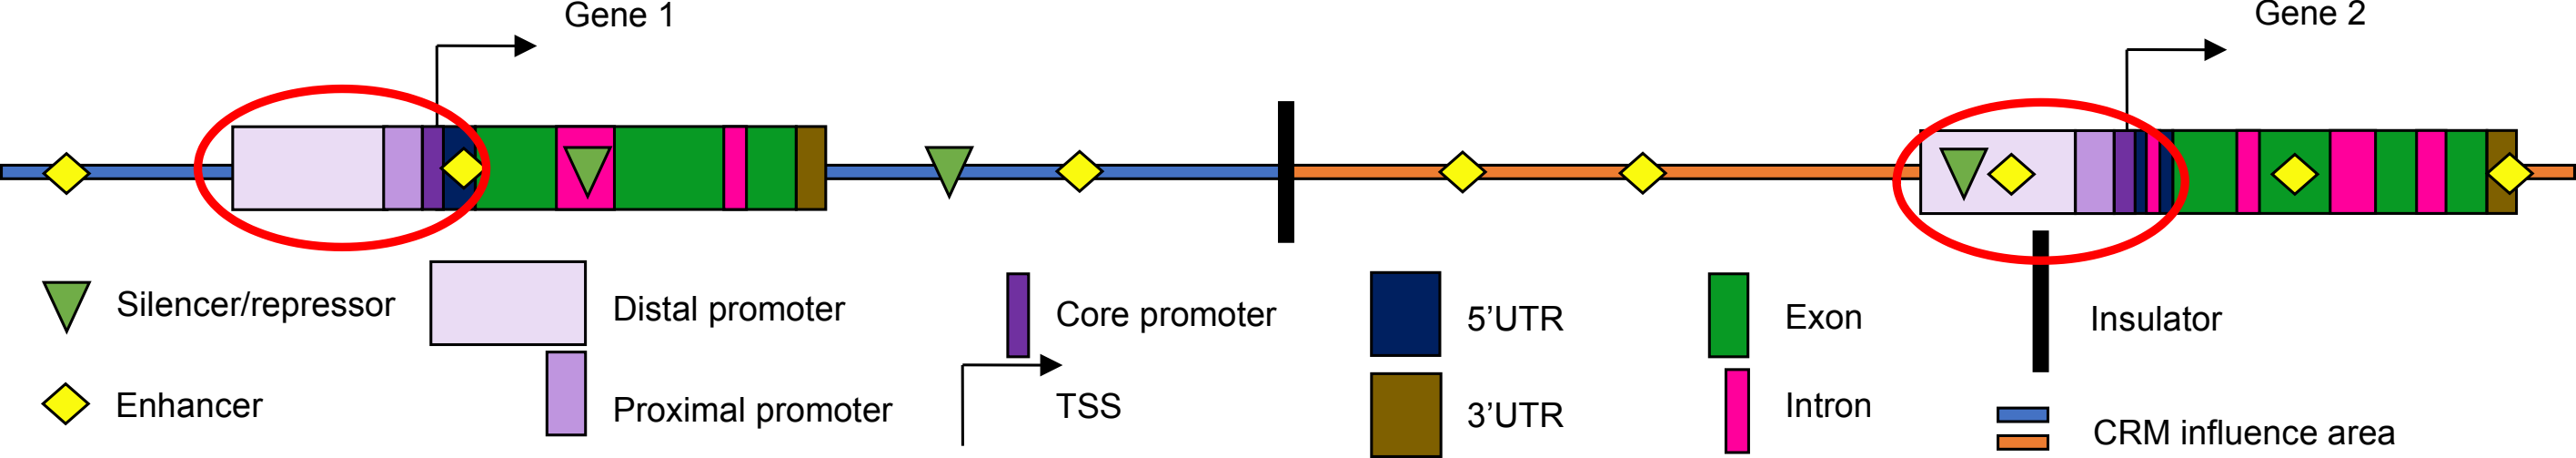
\includegraphics[width=0.70\columnwidth]{crm/crm}
\caption{\textit{Cis}\hyp{}regulatory module (CRM) classification. CRMs are genomic DNA
regions containing multiple \textit{cis}\hyp{}regulatory elements such as
transcription factor binding sites, which together regulate gene
transcription. UTR, untranslated region. CRMs include promoters,
silencers and insulators, and can be found within exons, introns, 3'UTRs
and 5'UTRs. CRM regulation is combinatorial, and can be unique to a
specific gene or shared between many. Insulators prevent CRMs from
regulating past that region. Transcription start sites (TSSs) are found
within the core promoter.
\label{fig:crm}
}
\end{center}
\end{figure}


\paragraph{The promoter}\label{The-promoter}
Promoters are essential in establishing baseline transcriptional capacity through the recruitment of proteins such as transcription factors (TFs), which control the recruitment of RNA polymerase II \autocite{portoPlantPromotersApproach2014}.
Promoters can be divided into two classes depending on when and where they are expressed.
Promoters active throughout the majority of developmental stages and environments are classed as constitutive promoters, and those only active in particular tissues (tissue\hyp{}specific) or in response to specific stimuli (inducible) can be termed variable promoters \autocite{bilasCisregulatoryElementsUsed2016}.
TFs bind CREs in a promoter to regulate the spatio\hyp{}temporal pattern of transcription of the downstream gene.
The promoter region can be split into three parts: core, proximal and distal.
The minimal DNA sequence required for transcription initiation is called the core promoter and this is usually spans from -60 to +40 bp relative to the transcription start site (TSS) \autocite{solovyevIdentificationPromoterRegions2010,royCorePromotersTranscription2015}.
\textit{Cis}\hyp{}regulatory elements (CREs) such as the initiator (Inr), TATA box and B recognition Element (BRE) are located in the core promoter.
Motif discovery\hyp{}based analyses hypothesised that general sequence enrichments in the core promoter of plants such as GA elements, CA elements and pyrimidine (Y)\hyp{}patch elements might have a similar function to mammalian promoter CpG (CG) islands \autocite{yamamotoCharacteristicsCorePromoter2011,yamamotoHeterogeneityArabidopsisCore2009}.
CpG sites in CpG islands are unmethylated when genes are expressed, and methylation in CpG sites can silence genes \autocite{birdDNAMethylationPatterns2002}.
In animals, TATA boxes are enriched in variable promoters~\autocite{engstromGenomicRegulatoryBlocks2007,carninciGenomewideAnalysisMammalian2006}, while CpG islands are enriched in constitutive promoters.
Additionally, mammalian constitutive promoters have a higher GC content than responsive promoters~\autocite{vinogradovDNAHelixImportance2017, weiCharacterizationGenePromoters2019}.
The proximal promoter region typically extends ~200\hyp{}300 bp upstream of the TSS and includes the part of the core promoter upstream of the TSS. The proximal promoter region also includes CREs for proteins including transcription factors.
The distal promoter can extend several 1000 bp upstream of the proximal promoter, and contains more CREs. However, these often have weaker influence on transcription than those in the proximal \autocite{pandiarajanVivoPromoterEngineering2018}.

\textcite*{mortonPairedEndAnalysisTranscription2014} used paired\hyp{}end analysis of TSSs (PEAT) to create a
dataset of TSSs from \textit{Arabidopsis thaliana} root samples. This
dataset was used to create a machine learning model called the Plant
PEAT Peaks (3PEAT) model, which predicts the TSS probability at any
given nucleotide. The majority of core plant promoters were found to be
TATA\hyp{}less, and instead contained many other CREs. \textcite*{thieffryCharacterizationArabidopsisThaliana2020} conducted cap\hyp{}analysis gene expression (CAGE) in Arabidopsis which agreed with \SI{95}{\percent} of the PEAT TSSs and was also more sensitive at
detecting more lowly expressed TSSs. Many core promoters contain a
cluster of multiple TSSs called the transcription start region (TSR)~\autocite{carninciGenomewideAnalysisMammalian2006,rachMotifCompositionConservation2009,niPairedendSequencingStrategy2010}. TSRs can be split into classes based on how wide a
region they cover in the core promoter. Narrow regions are associated
with strong, spatio\hyp{}temporal expression, and broader regions with the
weaker expression often associated with constitutively expressed
maintenance genes~\autocite{mortonPairedEndAnalysisTranscription2014}.

\paragraph{The enhancer}\label{the-enhancer}

Enhancers increase promoter activity, improving the spatio\hyp{}temporal
specificity of transcription in their target genes. Like promoters,
enhancers are DNA sequences that can contain many CREs recruiting a
variety of TFs and ncRNAs. Enhancers help activate transcription
regardless of their location, orientation or distance from promoters of
genes~\autocite{banerjiExpressionBetaglobinGene1981} (\autoref{fig:crm}). There
are several models explaining how enhancers work: (i) The proteins bound
to enhancers and promoters interact with each other by looping out the
DNA in between them~\autocite{carterLongrangeChromatinRegulatory2002,tolhuisLoopingInteractionHypersensitive2002,vilarDNALoopingGene2005,delaatChapterThreeDimensional2008,amanoChromosomalDynamicsShh2009}.
These interactions form the
transcription initiation protein complexes. This model is the most
highly accepted model. (ii) Enhancers can act by nucleosome remodelling,
supercoiling of DNA, and altering chromatin structure, facilitating the
entry of regulatory proteins to activate transcription~\autocite{corlessEffectsDNASupercoiling2016}. (iii) It has been suggested that both enhancers and
promoters share a common regulatory code, with transcription being
initiated at both~\autocite{coreNascentRNASequencing2008,engreitzLocalRegulationGene2016}. RNA polymerase II binds the core
promoter where it transcribes DNA in both the sense and antisense
directions. This is called bidirectional transcription. At promoters
this typically yields long, stable polyadenylated transcripts in the
sense direction, and short, unstable non\hyp{}polyadenylated transcripts in
the antisense direction~\autocite{anderssonPromoterEnhancerWhat2015}. At enhancers, unstable RNAs
called enhancer RNAs are produced in both directions~\autocite{dingEnhancerRNAsERNAs2018}.
These ncRNAs, along with cohesin, can stabilise long range
enhancer\hyp{}promoter interactions~\autocite{oromLongNoncodingRNAs2010}. In addition, introns
containing enhancers can sometimes be more important than the promoter
for initiating transcription~\autocite{gallegosIntronDNASequences2017}. In \textit{Drosophila}, two
classes of enhancers were identified that were specific to either
constitutively expressed promoters and variable promoters respectively~\autocite{zabidiEnhancerCorepromoterSpecificity2015}.
More than one enhancer can loop to the same promoter, and promoters with more enhancer loop interactions were more conserved than promoters forming fewer enhancer interactions~\autocite{dankoDynamicEvolutionRegulatory2018a}.

\paragraph{The 5'-untranslated region}\label{the-5-untranslated-region}

In protein coding genes, the 5'UTR is the stretch of DNA found between a
TSS and the translation start codon. This region is transcribed into
mRNA but is not translated into protein. Plant 5'UTRs can contain a
pyrimidine\hyp{}rich region (5'UTR Py\hyp{}rich stretch) which greatly improves
the transcription rate~\autocite{choudhuryComparativeStudyCultivar2009,duIsolationFunctionalCharacterization2010,bianCloningExpressionCharacterization2011}.
The 5' ends of the mRNAs are
processed by the replacement of the free triphosphate group with a
guanosine triphosphate. Once in place, this 5' cap plays a role in the
recognition of the mRNA by the ribosome~\autocite{byszewskaRNAMethyltransferasesInvolved2014,ramanathanMRNACappingBiological2016}. The mRNAs of
mitochondria~\autocite{temperleyHumanMitochondrialMRNAs2010} and chloroplasts~\autocite{mondeProcessingDegradationChloroplast2000} are
not capped. Once transcribed, the 5'UTR sequence can contain an upstream
open reading frame (uORF) (\SI{50}{\percent} of human 5'UTRs do)~\autocite{calvoUpstreamOpenReading2009},
a guanine\hyp{}rich region~\autocite{beaudoinUTRGquadruplexStructures2010} and an internal ribosome entry
site (IRES)~\autocite{jimenez-gonzalezFunctionalStructuralAnalysis2014}.
Alternative 5'UTRs can be produced via alternative splicing or through
transcription initiation from a different TSS~\autocite{smithPosttranscriptionalRegulationGene2008}.
Because current TSS annotations in the Arabidopsis genome~\autocite{lameschArabidopsisInformationResource2012} are not accurate~\autocite{mortonPairedEndAnalysisTranscription2014,thieffryCharacterizationArabidopsisThaliana2020} and the 5'UTR may contain CREs, it is important to include the 5'UTR in regulatory sequence studies to encompass the whole TSR.

\subsubsection{\textit{Trans}-acting DNA regulation}\label{trans-acting-dna-regulation}

A \textit{trans}\hyp{}regulatory sequence is a DNA sequence that contains a
gene encoding for a protein or ncRNA that is used in the regulation of
another target gene~\autocite{watsonRecombinantDNAGenes2007}. \textit{Trans}\hyp{}acting regulation
can involve the specific binding of a \textit{trans}\hyp{}acting molecule such
as a TF or ncRNA to a DNA CRE. Another form of \textit{trans}\hyp{}acting
regulation involves non\hyp{}specific DNA binding by molecules such as
eukaryotic histone proteins in nucleosomes~\autocite{zhangIntrinsicHistoneDNAInteractions2009}.

\paragraph{Sequence specific \textit{trans}-regulation}\label{sequence-specific-trans-regulation}

TFs are \textit{trans}\hyp{}acting proteins with domains which bind to TFBSs in
DNA. ncRNAs can contain DNA binding domains which form triple helices
with certain \textit{cis}\hyp{}regulatory elements called triplex target sites
(TTS)~\autocite{kuoDetectionRNADNA2019}. TFs and ncRNAs can contain domains which
interact with other proteins to form complexes which can enhance or
repress gene transcription. Some TFs are able to bind DNA as both
homodimers and heterodimers, increasing regulatory combinations. DNA
regulatory modules such as enhancers can be found on different
chromosomes to the gene they are regulating, where they function in
\textit{trans}~\autocite{geyerTissuespecificTranscriptionalEnhancers1990,xuTransientHomologousChromosome2006,lomvardasInterchromosomalInteractionsOlfactory2006}.

TFs are often part of large families, and many TFs within the same
family can bind to highly overlapping sets of binding sites. TFs from
different families such as bZIPs and bHLHs can compete to bind the same
TFBS~\autocite{toledo-ortizHY5PIFRegulatoryModule2014}. Change in the expression of one TF can
result in cross talk, where the expression of gene targets of other TFs
from the same family are also altered~\autocite{nuruzzamanRolesNACTranscription2013}. Plant TF
families have higher expansion rates than other eukaryotes, not only due
to genome duplications, but also due to increased retention of duplications
within TF families compared to other plant genes~\autocite{shiuTranscriptionFactorFamilies2005}.

An important aspect of TF\hyp{}DNA interactions is the DNA shape. Most
DNA\hyp{}protein interactions occur in the major groove, where bases are most
accessible~\autocite{paboProteinDNARecognition1984}, although some occur in the minor groove~\autocite{bewleyMinorGroovebindingArchitectural1998}. TFs undergo rapid rebinding to ensure the correct orientation is achieved during docking to DNA~\autocite{ganjiDNABindingProteins2016}. The
DNA base cytosine can be methylated, becoming 5\hyp{}methylcytosine (5mC). By
comparing TF binding affinity to TFBSs with and without 5mC, it has been
suggested that TFs might belong to three main groups: (i)
methylation\hyp{}inhibited, (ii) methylation\hyp{}insensitive and (iii)
methylation\hyp{}preferred \autocite{huangPiecingTogetherCisregulatory2018}. Out of \SI{30}{\percent} of
Arabidopsis TFs studied, \SI{76}{\percent} were sensitive to methylation in
their corresponding TFBSs~\autocite{omalleyCistromeEpicistromeFeatures2016}. In a GRN it is important
to incorporate the sequence specific interactions between
\textit{trans}\hyp{}acting molecules, and also between themselves and
regulatory regions in DNA to better understand how to manipulate
networks.

\paragraph{Chromatin}\label{chromatin}

Eukaryotic genomes are packed into chromatin, a complex of protein, RNA
and DNA~\autocite{mondalCharacterizationRNAContent2010}, made up of repeating units called
nucleosomes consisting of a histone octamer wrapped around by \num{146} or \num{147}
bp of DNA~\autocite{richmondStructureDNANucleosome2003}. Many DNA CRMs such as promoters and
enhancers are depleted of nucleosomes and some are nucleosome
free~\autocite{struhlDeterminantsNucleosomePositioning2013}. In gene regulatory studies it is important to
incorporate data on non\hyp{}sequence specific interactions between
\textit{trans}\hyp{}acting molecules (\eg{} nucleosome histone proteins) and DNA,
as they reduce how accessible DNA is to other \textit{trans}\hyp{}acting
molecules. Nucleosomes can inhibit the access of TFs to TFBSs. Chromatin
regions highly accessible to DNA\hyp{}binding proteins are called
deoxyribonuclease (DNase) I hypersensitive sites (DHSs) and these can be
mapped following DNase I digestion.

A class of pioneer TFs are able to bind their targets in the presence of nucleosomes.
These pioneer TFs recruit nucleosome remodelers to open up chromatin, allowing previously blocked TFs access to the region~\autocite{zaretPioneerTranscriptionFactors2011}.
In yeast (\textit{Saccharomyces cerevisiae}), stiff DNA poly(dA:dT) regions~\autocite{yuanGenomeScaleIdentificationNucleosome2005,hughesFunctionalEvolutionaryApproach2012} and poly(dG:dC) regions~\autocite{mccallCrystalStructureGGGGCCCC1985} were shown to be depleted of nucleosomes, whereas non\hyp{}homopolymeric GC\hyp{}rich regions favour nucleosome formation~\autocite{struhlDeterminantsNucleosomePositioning2013}.
Yeast promoters containing GC\hyp{}rich motifs and poly(A) motifs concentrated in a narrow region tend to be nucleosome free.
Promoters with the same two motifs in a broader region are characterised by `fragile' nucleosomes, which are less stable.
Fragile nucleosome promoters tend to be highly expressed.
The two motifs have been shown to recruit and/or activate the chromatin structure remodelling complex (RSC) which pushes away flanking nucleosomes, creating a nucleosome free region or space for a fragile nucleosome to form.
To induce nucleosome fragility, Rap1 binding sites were needed upstream of the GC\hyp{}rich and poly(A) motifs~\autocite{kubikNucleosomeStabilityDistinguishes2015}.
Fragile nucleosomes have been detected in maize~\autocite{veraDifferentialNucleaseSensitivity2014} and Arabidopsis~\autocite{passGenomewideChromatinMapping2017}.

\subsubsection{Identification of CREs}\label{identification-of-cres}

In order to understand how DNA\hyp{}protein interactions affect gene function it is necessary to understand which proteins bind to specific binding sites in DNA.
Earlier methods involved \textit{in vitro} techniques, however more recent studies identify sites bound by proteins \textit{in vivo}, preserving both context and DNA sequences involved.
A recent \textit{in vitro} method~\autocite{omalleyCistromeEpicistromeFeatures2016} maps protein\hyp{}DNA interactions using DNA retaining \textit{in vivo} features.
Mapping chromatin accessibility and TFBSs helps inform our understanding of gene regulation, and therefore is the basis of understanding and reconstructing gene regulatory networks.

\subsubsection{Identification of chromatin accessible
regions}\label{identification-of-chromatin-accessible-regions}

In the past, it was difficult to annotate non\hyp{}coding DNA regions, and at the genomic scale it was only possible to detect the presence or absence or `regulatory regions'.
As detailed in section \ref{chromatin} (chromatin), CRMs tend to be nucleosome free regions, are very sensitive to digestion by DNase I, and are called DHSs. Many DHS assays have been used to characterise CRMs.
Chromatin accessibility of DNA to DNase I was probed by Southern blotting where, following DNase I digestion, DNA was purified, digested using restriction enzymes, transferred to a membrane then hybridised with radioactively labelled DNA~\autocite{wuChromatinStructureSpecific1979,matherMethylationStatusDNase1983,benderVglobinGeneSwitching2000,wangChromatinStructureMapping2001}.
This was challenging, limited to short stretches of DNA and not very sensitive~\autocite{cockerillIdentificationDNaseIHypersensitive2000}.
DHS methods using PCR (polymerase chain reaction)~\autocite{pfeiferChromatinDifferencesActive1991,fengHighresolutionAnalysisCfos1992} and later quantitative PCR (qPCR)~\autocite{mcarthurQuantificationDNaseIsensitivityRealtime2001,dorschnerHighthroughputLocalizationFunctional2004,martinsTrackingChromatinStates2007} were developed to improve upon the Southern blotting technique for identification of chromatin accessible regions.
DNase I assays were combined with genome\hyp{}wide tiling arrays (DNase-chip) with sequencing~\autocite{crawfordIdentifyingGeneRegulatory2004,saboGenomewideIdentificationDNaseI2004}, and without sequencing~\autocite{crawfordDNasechipHighresolutionMethod2006,saboGenomescaleMappingDNase2006,followsIdentifyingGeneRegulatory2006,shuDistinctModesDNA2012} for genome\hyp{}wide profiling of chromatin accessibility.

As an alternative to DNase assays, a high\hyp{}throughput assay later called formaldehyde\hyp{}assisted isolation of regulatory elements (FAIRE) was developed~\autocite{nagyGenomewideDemarcationRNA2003}.
In this assay, formaldehyde\hyp{}crosslinked chromatin and reference non\hyp{}crosslinked chromatin is extracted using phenol\hyp{}chloroform.
Histone\hyp{}free DNA is collected in the aqueous phase, and enrichment of histone\hyp{}free DNA regions from crosslinked DNA are identified by comparing to the non\hyp{}crosslinked reference on a microarray.

More recent methods combine high\hyp{}throughput sequencing with previous methods, such as DNase-chip with sequencing (DNase I-seq)~\autocite{boyleHighResolutionMappingCharacterization2008} and the FAIRE assay with sequencing (FAIRE-seq)~\autocite{giresiFAIREFormaldehydeAssistedIsolation2007}.
Although DNase-chip was previously combined with sequencing~\autocite{crawfordGenomewideMappingDNase2006}, this only identified \SI{20}{\percent} of DHS sites. Higher throughput sequencing allowed production of genome wide DHS maps~\autocite{boyleHighResolutionMappingCharacterization2008}.
The combination of DNase I-seq with FAIRE-seq to map open chromatin is more effective than either assay alone~\autocite{songOpenChromatinDefined2011}.
DNase I-seq and FAIRE-seq require millions of cells as starting material, with time\hyp{}consuming sample preparations.
This means heterogeneity between cells can be drowned out.
To improve on this, genome\hyp{}wide DNase I-seq has since been scaled down to single cells, called scDNase-seq~\autocite{jinGenomewideDetectionDNase2015}.

The assay for transposase\hyp{}accessible chromatin using sequencing (ATAC\hyp{}seq)~\autocite{buenrostroTranspositionNativeChromatin2013} was developed to require fewer cells in the starting material.
ATAC\hyp{}seq identifies nucleosome\hyp{}bound and nucleosome free regions, along with footprinting of DNA binding proteins.
This method builds on the fact that transposons were shown to integrate into active regulatory regions \textit{in vivo}~\autocite{gangadharanDNATransposonHermes2010}, and uses Tn5 transposase to integrate its adaptor payload into DNA within chromatin accessible regions. ATAC\hyp{}seq uses a simple two\hyp{}step process of Tn5 insertion followed by PCR and sequencing, whereas FAIRE\hyp{}seq and DNase I\hyp{}seq have many more steps and take several days~\autocite{buenrostroTranspositionNativeChromatin2013}.
Single cell ATAC\hyp{}seq (scATAC\hyp{}seq) has also been achieved~\autocite{cusanovichMultiplexSinglecellProfiling2015,buenrostroSinglecellChromatinAccessibility2015}.
The cutting bias of DNase I in DNase I\hyp{}seq~\autocite{heRefinedDNaseseqProtocol2014} and Tn5 transposase in ATAC\hyp{}seq~\autocite{martinsUniversalCorrectionEnzymatic2018} needs to be corrected computationally when analysing data~\autocite{liuLongNoncodingRNA2019a}.

ATAC\hyp{}seq and DNase I\hyp{}seq identify regions of open chromatin which correlate to nucleosome occupancy.
Nucleosome occupancy itself can be profiled genome\hyp{}wide using micrococcal nuclease digestion followed by sequencing (MNase\hyp{}seq) \autocite{weberH2ANucleosomesEnriched2010,henikoffEpigenomeCharacterizationSingle2011,pajoroProfilingNucleosomeOccupancy2018}.
In Mnase\hyp{}seq, DNA is digested using MNase unless it is protected by nucleosomes.
Protected DNA can then be sequenced in a high\hyp{}throughput manner to identify nucleosome sites.
An alternative to MNase\hyp{}seq called NOMe\hyp{}seq (nucleosome occupancy and methylome sequencing)~\autocite{kellyGenomewideMappingNucleosome2012} uses GpC methyltransferase which methylates GpC dinucleotides not protected by nucleosomes or strongly binding proteins.
Native methylation uses CpG dinucleotide cytosine methylation, whereas the added GpC methyltransferase methylates GpC dinucleotide cytosines.
Using this information, both nucleosome occupancy and endogenous DNA methylation can be obtained simultaneously.

\subsection{Identification of specific DNA-protein
interactions}\label{identification-of-specific-dna-protein-interactions}

DNase I is used to footprint DNA\hyp{}protein interactions.
\textit{In vitro} DNase I footprinting is where radioactively labelled DNA fragments are incubated with and without the protein of interest, then digested with DNase I and analysed by electrophoresis and autoradiography~\autocite{galasDNAseFootprintingSimple1978}.
Bound proteins protect the DNA backbone from digestion by DNase I, allowing identification of specific binding sites of proteins on DNA.
Another method for characterising DNA\hyp{}protein interactions is the electrophoretic mobility shift assay (EMSA)~\autocite{garnerGelElectrophoresisMethod1981}, which quantifies the binding of proteins to DNA.
A fragment of DNA containing a putative TFBS is fluorescently or radioactively labelled and is run on a polyacrylamide gel with and without the protein of interest.
DNA\hyp{}protein complexes run more slowly on the gel than DNA on its own.

More recent techniques include systematic evolution of ligands by exponential enrichment (SELEX).
SELEX is an \textit{in vitro} assay where libraries of randomly generated nucleic acid ligands of fixed length are flanked by 5' and 3' primers~\autocite{tuerkSystematicEvolutionLigands1990}.
The oligonucleotide library is exposed to a protein of interest, unbound oligos are removed, and then oligos are amplified using PCR.
This cycle is repeated several times until the oligo population is enriched for ones which bind protein.
These are then identified and characterised.
SELEX has recently been modified to investigate the location and orientation of TFBSs in DNA wrapped around nucleosomes, with a technique called nucleosome consecutive affinity purification (NCAP)\hyp{}SELEX~\autocite{zhuInteractionLandscapeTranscription2018}.
This uses SELEX to enrich nucleosome bound DNA, and then DNA is incubated with TFs.
Using nucleosome and TF tags, DNA is separated based on whether or not it is bound by nucleosomes and TFs, and is then sequenced.
This infers whether the addition of a certain TF affects the stability of the nucleosome, and identifies TF binding specificities and positions on nucleosomal DNA.

Chromatin immunoprecipitation (ChIP) was developed to map protein\hyp{}DNA crosslinking \textit{in vivo}.
There are two types of ChIP, differentiated by starting input.
XChIP uses chromatin fixed with formaldehyde and sheared by sonication~\autocite{solomonMappingProteinDNAInteractions1988,orlandoMappingChromosomalProteins2000}, and NChIP uses native chromatin from nuclei digested by micrococcal nuclease~\autocite{hebbesDirectLinkCore1988}.
Protein specific antibodies are then used to pull down the protein of interest bound to DNA.
The resulting DNA sequences are then purified and analysed using Southern blot, PCR or qPCR~\autocite{dasChromatinImmunoprecipitationAssay2004}, although PCR bias may mean AT\hyp{}rich sequences are amplified more than GC\hyp{}rich ones~\autocite{weinmannIdentificationUnknownTarget2002}.
NChIP is most useful for mapping the DNA target of histone modifiers, while XChIP is most useful for mapping TF\hyp{}DNA interactions.
Even so, some TF\hyp{}DNA interactions have been successfully mapped using NChIP~\autocite{gregoryDNAMethylationLinked2001}.
ChIP has been combined with sequencing to identify DNA sequences where proteins bind~\autocite{weinmannUseChromatinImmunoprecipitation2001}, and also combined with DNA footprinting, to identify specific TFBSs~\autocite{leekangCombiningChromatinImmunoprecipitation2002}.
Although these methods accurately identify TFBSs in DNA, a drawback is that they are very low throughput.

To increase throughput, ChIP was combined with whole\hyp{}genome microarrays (ChIP\hyp{}chip), creating high resolution genome wide maps of DNA\hyp{}protein interactions~\autocite{weinmannIsolatingHumanTranscription2002,wellsIdentificationNovelPRb2003,renGenomeWideLocationFunction2000}.
\textcite*{buckChIPchipConsiderationsDesign2004} provide an excellent review of this.
Briefly, XChIP is carried out, and DNA fragments enriched for protein binding are purified and fluorescently labelled.
Genomic DNA prepared by immunoprecipitation is used as a reference, amplified, and labelled with a different tag.
The two probes are hybridised onto a single DNA microarray.
Areas of the genome enriched for DNA\hyp{}protein binding are identified, and exact binding sites can be predicted \textit{in silico}~\autocite{liuAlgorithmFindingProtein2002}.

ChIP\hyp{}chip is limited in that only a subset of TFBSs are retrieved due to the array design.
Also, ChIP\hyp{}chip is restricted to species for which whole\hyp{}genome tiling arrays have been made.
With the advance of high\hyp{}throughput sequencing technology, these limitations were overcome through the development of ChIP\hyp{}seq, where ChIP DNA is sequenced in a high\hyp{}throughput way, providing greater sensitivity, resolution and specificity than ChIP\hyp{}chip~\autocite{johnsonGenomeWideMappingVivo2007}.

ChIP\hyp{}seq provides genome\hyp{}wide TFBS mapping for specific TFs.
Even so, TFBS information is available for relatively few TFs.
This is because ChIP\hyp{}seq is not scalable for high\hyp{}throughput identification of 1000s of TF\hyp{}DNA interactions as it is dependent on antibody quality, is difficult for lowly expressed proteins and is challenging to perform~\autocite{kidderChIPSeqTechnicalConsiderations2011}.

Another method of identifying DNA-protein interactions is DNA adenine methyltransferase identification (DamID)~\autocite{steenselIdentificationVivoDNA2000}. DamID uses the \textit{E. coli} DNA adenine methyltransferase (Dam) fused to a TF or chromatin protein of interest.
Wherever the protein of interest binds, even transiently, Dam methylates adenine in GATC motifs~\autocite{sanchez-romeroDNAMethylationBacteria2015}.
DNA is then extracted and fragmented by the methylation sensitive restriction endonuclease DpnI.
Methylated sequences are then amplified by PCR and then sequenced.
DamID and ChIP methods are fundamentally different.
DamID shows where a protein has previously been in close proximity to DNA, even transiently, while ChIP shows where a protein binds DNA at a given time point.
DamID is good for identifiying DNA-protein interactions which are low in abundance, while ChIP methods struggle to pick them up.
ChIP on the other hand is good for profiling DNA-protein interactions at short time intervals, while Dam-fusions require expression for several hours to achieve sufficient methylation~\autocite{augheyDamItGood2016}.

The protein binding microarray (PBM) is another method of identifying TF-DNA interactions developed by \textcite*{bulykProteinBindingMicroarrays2007}. In this method, a TF of interest is expressed with an epitope tag which is purified and then applied to a DNA microarray. Any non-bound protein is washed away and then the microarray is stained with a primary antibody specific to the epitope tag. The signal intensity can be quantified as it corresponds to the number of DNA-protein binding events. PBM analysis was utilised in Arabidopsis to identify DNA binding motifs for 63 TFs~\autocite{franco-zorrillaDNAbindingSpecificitiesPlant2014}.

The recently developed \textit{in vitro} DNA affinity purification sequencing (DAP-seq) offers a scalable alternative to ChIP and increased specificity compared to motifs generated by PBMs and SELEX~\autocite{omalleyCistromeEpicistromeFeatures2016}.
DAP\hyp{}seq uses \textit{in vitro} expressed TFs to find binding locations on genomic DNA retaining its \textit{in vivo} properties.
Briefly, a genomic DNA library is prepared by attaching a small DNA sequencing adaptor onto purified, fragmented genomic DNA.
Separately, affinity\hyp{}purified TFs are prepared by \textit{in vitro} expression.
The DNA library is added to each specific TF, and unbound DNA is washed away.
The bound fraction is amplified and sequenced.
Reads are mapped to a reference genome and enriched peaks are used to identify TFBSs.
As this uses genomic DNA, which contains cell, tissue and organism specific methylation, methylation preferences of TFs can be mapped.
This is done using a modified DAP\hyp{}seq protocol called ampDAP\hyp{}seq, where a DNA library has any modifications removed by use of a PCR step.
This data can be compared to DAP\hyp{}seq data to assess the methylation preferences of TF binding~\autocite{omalleyCistromeEpicistromeFeatures2016}.

Methods like ChIP, DamID, PBMs and DAP-seq are TF\hyp{}centred methods.
The yeast one\hyp{}hybrid (Y1H) assay is a DNA centred method to identify proteins binding the DNA~\autocite{liIsolationORC6Component1993}.
It involves a report construct where the promoter DNA of interest (termed the bait) is placed upstream of a reporter protein.
A TF of interest (termed the prey) is fused to a yeast transcription activation domain and is expressed in an expression construct.
Both constructs are introduced to a yeast strain, and if the TF of interest binds the DNA of interest then the yeast activator domain induces the reporter expression.
The downside of Y1H assays is that they do not identify whether a TF of interest activates or represses a promoter~\autocite{reece-hoyesYeastOnehybridAssays2012}.
The throughput of Y1H assays were enhanced using a robotic mating platform~\autocite{reece-hoyesEnhancedYeastOnehybrid2011}.
Recently, this enhanced Y1H assay was used in plants to elucidate interactions between nitrogen-responsive genes~\autocite{gaudinierTranscriptionalRegulationNitrogenassociated2018}.

The \textit{in vitro} techniques such as DAP-seq, Y1H and PBMs fail to account for \textit{in vivo} features such as chromatin structure, protein-protein interactions and TF combinations.
The \textit{in vivo} method ChIP does not show whether a TF-DNA interaction leads to gene expression, and it often poorly predicts TF regulation~\autocite{brooksNetworkWalkingCharts2019}.
TF perturbation using overexpressing or knockout transgenic lines are one way of validating targets but these methods are time consuming and do not scale well in eukaryotes.
It is also not possible to distinguish direct from indirect targets.
A technique called transient assay reporting genome\hyp{}wide effects of transcription factors (TARGET) was developed in plant protoplasts~\autocite{bargmannTARGETTransientTransformation2013}.
Briefly, the TF of interest is fused to a glucocorticoid receptor (GR) and expressed transiently in protoplasts.
The expression plasmid also contains a separate expression cassette with red fluorescent protein (RFP) enabling fluoresence\hyp{}activated cell sorting (FACS) of transformed protoplasts~\autocite{bargmannFluorescenceActivatedCell2010}.
The GR-TF fusion is held in the cytoplasm by HSP90-GR binding. Dexamethasone (DEX) is added which disrupts the HSP90-GR binding and induces nuclear localisation of the TF.
Target gene induction after DEX treatment with and without the presence of a translation inhibitor, cycloheximide (CHX), is measured using qPCR analysis.
This shows direct and indirect gene regulation.
Recently, the TARGET method was scaled up using an empty vector control allowing 24 TF assays per day (8 TFs with 3 replicates)~\autocite{brooksNetworkWalkingCharts2019}.
All samples including the empty vector were treated with CHX, mitigating the need to compare CHX positive and negative samples.
Cells separately transfected with either RFP or green fluorescent protein (GFP) were pooled in pairs, allowing the simultaneous FACS of two TFs in each well.
After FACS, RNA-seq analysis was used to identify activated or repressed targets.
However, this scaled up method only detects direct targets.
It is necessary to combine TF-target methods to fully illucidate connections in GRNs.
A time\hyp{}series micro-ChIP protocol for use with small cell samples~\autocite{dahlMChIPRapidMicro2008} was modified for use with the TARGET assay~\autocite{paraMChIPSeqGenomeWideMapping2018} allowing both methods to be run on the same samples~\autocite{paraHitandrunTranscriptionalControl2014, doidyHitandRunTranscriptionNovo2016}.
A recent study combined micro-ChIP, DamID and the TARGET assay allowing transiently bound targets of the NLP7 TF to be identified five minutes after nuclear localisation of the TF~\autocite{alvarezTransientGenomewideInteractions2020}.
These studies also utilised 4-thiouracil (4tU) labelling of nascent transcripts~\autocite{sidaway-leeDirectMeasurementTranscription2014}, allowing affinity-based capture of \textit{de novo} synthesised RNA.
By monitoring TF-DNA interactions over time and using 4tU labelling and steady\hyp{}state RNA-seq these two methods showed that targets of bZIP1 and NLP7 continued to be actively transcribed even after the TFs dissociated from their targets.

In Arabidopsis, recent DNase I\hyp{}seq data~\autocite{sullivanMappingDynamicsRegulatory2014} was published, predicting active regulatory regions where many TFs can bind.
The development of DAP\hyp{}seq has characterised specific TFBSs from a third of Arabidopsis TFs~\autocite{omalleyCistromeEpicistromeFeatures2016}.
Therefore, TFBS data can now be overlayed with the DNase I\hyp{}seq footprint data to map regulatory regions in Arabidopsis.
TFBSs can also be predicted \textit{de novo} with software that can construct position weight matrices (PWMs) describing the binding motifs of a TFs, such as MEME~\autocite{baileyFittingMixtureModel1994}, and the faster STEME~\autocite{reidSTEMEEfficientEM2011}.
Motif prediction has a high false positive rate~\autocite{zambelliMotifDiscoveryTranscription2013}.
Algorithms such as RPMCMC~\autocite{ikebataRepulsiveParallelMCMC2015} and DREME~\autocite{baileyDREMEMotifDiscovery2011} offer cofactor motif discovery, which for example can predict whether TFs form homo and heterodimers when they bind.
In 2015, convolutional neural network (CNN) models were able to learn filters similar to PWM motif matching, and these algorithms outperformed PWM algorithms~\autocite{alipanahiPredictingSequenceSpecificities2015}.
An unpublished CNN model incorporates TF\hyp{}TF interactions during its TFBS prediction~\autocite{lanchantinPrototypeMatchingNetworks2017}.

\subsection{Evolution of gene regulation}
{\label{evolution-of-gene-regulation}}

Investigations into the DNA conservation landscape have identified
conserved DNA regions within populations and across species, and this is
because of selection pressure. Evolutionary selection pressure is higher
for coding exon sequences than it is for non\hyp{}coding regulatory sequences
such as the promoter, 5' and 3'UTRs in mammals~\autocite{lindblad-tohHighresolutionMapHuman2011} and
plants~\autocite{haudryAtlas900002013}. However, functional motifs such as TFBSs
within non\hyp{}coding regions exhibit high levels of evolutionary
conservation~\autocite{zhaoConservedMotifsPrediction2012}. When these functional motifs change,
for example due to random mutations called single nucleotide
polymorphisms (SNPs), they can cause changes in expression
level~\autocite{rockmanAbundantRawMaterial2002} and potentially even network
rewiring~\autocite{liEvolutionTranscriptionNetworks2010}. This can be through a change in the
affinity of TFs to the TFBS, addition or deletion of sites, change in
the spacing of TFBSs, or change in nucleosome conformation in the area~\autocite{fyonEnhancerRunawayEvolution2015}.

Some genes may have multiple copies in the genome, which express
products with similar functions~\autocite{guRapidDivergenceExpression2002}. In redundant copies,
the selection pressure on motifs in their non\hyp{}coding regions may be
reduced, resulting in random mutations accumulating in the motifs. These
gene copies therefore may have different spatio\hyp{}temporal expression
patterns~\autocite{forcePreservationDuplicateGenes1999}. These different expression patterns could
have evolved following genome expansion. New genes can be formed through
evolutionary whole genome duplications, creating ohnologues.
Additionally, small\hyp{}scale duplications (SSDs) can occur. One such
example is tandem duplication, which creates consecutive gene copies in
the genome due to unequal crossing over~\autocite{freelingBiasPlantGene2009}. Other SSDs
include retroposed duplicates, created through RNA\hyp{}mediated
retroposition; proximal duplicates, where duplicate genes are separated
by a few genes; and dispersed duplicates, where duplicates are found
throughout the genome, not in syntenic homologous chromosome
regions~\autocite{arsovskiEvolutionCisRegulatoryElements2015}.

There are two types of genetic events affecting gene regulation: (i)
those caused by point mutations of existing sequences, and (ii) those
caused by genome expansion driven by transposable elements, genome
duplications and small scale duplications (SSDs)~\autocite{marnettoEvolutionaryRewiringHuman2018}. Once duplicated, mutations can arise in one paralogue turning it into a
non\hyp{}functional pseudogene~\autocite{zhangEvolutionGeneDuplication2003}. If the original gene had
several functions, these can be shared between both paralogues, in a
process called subfunctionalisation. Regulatory subfunctionalisation can
occur where paralogues retain the same function but tissue specific
expression patterns become shared between them. Another possibility
following gene duplication is that one paralogue can acquire a new
function whilst the other maintains its original function, which is
called neofunctionalisation. In regulatory neofunctionalisation, one
paralogue acquires a novel expression pattern, while the other keeps its
original expression pattern. Duplicated genes can undergo both neo- and
subfunctionalisation~\autocite{heRapidSubfunctionalizationAccompanied2005}. Duplicated genes can also both
maintain ancestral function and expression pattern, adding to robustness
of their regulatory network~\autocite{guRoleDuplicateGenes2003}. However, gene
duplication can cause fragility in GRNs, instead of improving their
robustness. This may be he case if the function of the protein of one
paralogue becomes dependent on the presence of the other~\autocite{dissGeneDuplicationCan2017}. Hypofunctionalisation has also been proposed, where
the expression level of the paralogues decreases, meaning both copies
are required for normal function~\autocite{qianMaintenanceDuplicateGenes2010,veitiaGeneDuplicatesAgents2017}.

Mutations within CREs of duplicated genes are the likely cause of
regulatory neo- and subfunctionalisation~\autocite{arsovskiEvolutionCisRegulatoryElements2015}. Recently,
duplicated genes in yeast were shown to quickly gain TFBSs after
duplication~\autocite{tsaiEvolutionCisregulatoryElements2012}. Additionally, it has been suggested that
in all eukaryotic diploid organisms, enhancer strength may increase in a
runaway fashion due to the competition for expression between homologous
enhancer alleles~\autocite{fyonEnhancerRunawayEvolution2015}. In plants, the distribution of
known core promoter elements with respect to the TSS is conserved within
monocots and dicots~\autocite{kumariGenomeWideComputationalPrediction2013}.

\subsection{Engineering regulation}\label{engineering-regulation}

\subsubsection{Development of synthetic regulatory elements for
microbes}\label{development-of-synthetic-regulatory-elements-for-microbes}

Many studies have described the assembly and characterisation of
promoter libraries for microbes. For example, in \textit{E. coli} ,
directed evolution was used to engineer a broad range of precise
promoter strengths~\autocite{alperTuningGeneticControl2005}. Promoters made in this way tend
to have a broad host range~\autocite{jensenSequenceSpacersConsensus1998}. Combinatorial libraries
of random promoter architectures has also been achieved in \textit{E.
coli~}~\autocite{coxProgrammingGeneExpression2007}. They show that gene expression can be
regulated by over five orders of magnitude. The location of regulatory
elements within a promoter was key to determining the expression level,
with those located closer to the TSS more effective than those further
away. Some regulatory elements were dominant over others when located in
the same promoter. More directed semi\hyp{}rational promoter engineering
focussed on retaining the consensus sequence of TFBSs, and mutating
spacers~\autocite{jensenSequenceSpacersConsensus1998}. Rational promoter design increased \textit{E.
coli} promoter activity through the addition of a TFBS~\autocite{zhangDesignDynamicSensorregulator2012}. A synthetic promoter utilising an AND gate, where it
is only activated in the presence of two TFs, was also created
in \textit{E. coli}~\autocite{wangEngineeringModularOrthogonal2011}. A ratiometric expression assay was
used in \textit{E. coli} to characterise gene expression level, by
measuring activity of promoters compared to a reference, and variation
between experiments was reduced by \texttildelow\SI{50}{\percent} \autocite{kellyMeasuringActivityBioBrick2009}.

Synthetic promoter libraries in the yeasts \textit{Komagataella
pastoris}~\autocite{hartnerPromoterLibraryDesigned2008} and \textit{S. cerevisiae}~\autocite{nevoigtEngineeringPromoterReplacement2006} showed that promoter strength could be changed by introducing mutations in TFBSs. Synthetic promoters were used to study nucleosome occupancy
effects on transcription, and allowed the rational design of synthetic
promoters with increased transcription~\autocite{curranDesignSyntheticYeast2014}. A massively
parallel reporter assay (MPRA) was used to test semi\hyp{}random 312 bp
constitutive and 246 bp responsive promoters in \textit{S. cerevisiae},
where conserved regions containing TFBSs remained the same~\autocite{kotopkaModeldrivenGenerationArtificial2020}. Machine
learning facilitated the \textit{in silico} design of new promoters of
specific expression levels, including expression higher than in any of
the test data set used to train the model. When tested \textit{in
vivo} these designed promoters had similar expression levels to the
predicted values. Synthetic minimal yeast promoter
libraries were generated to identify minimal upstream activating
elements, and this led to the development of a promoter reduced by \SI{80}{\percent}
in size which still achieved high expression levels~\autocite{reddenDevelopmentCharacterizationSynthetic2015}.

The use of synthetic TFs allows control of gene expression
heterologously in many systems, and allows the design of tissue specific and
or constitutive promoters, as synthetic TFs can themselves be controlled
by tissue specific or constitutive promoters. Synthetic TFs have been
created in yeast using zinc fingers~\autocite{khalilSyntheticBiologyFramework2012}, with a
methodology allowing construction of an unlimited number of different
synthetic TFs. Transcriptional output was tuned through modification of
zinc finger binding sites in promoters, as well as through modifications
to the zinc finger protein itself. Later, inducible synthetic
transcription activator\hyp{}like effectors (TALEs) and dCas9\hyp{}based synthetic
TFs together with small synthetic promoters were trialled, also in yeast~\autocite{machensSyntheticPromotersTranscription2017}. Synthetic TFs have been designed using zinc fingers in \textit{E. coli} too~\autocite{husseyProgrammableT7basedSynthetic2018}. This enabled activation of promoters, rather than de\hyp{}repression of promoters which had been used in
the past, as bacterial promoters are generally on by default~\autocite{browningLocalGlobalRegulation2016}.

\subsubsection{Synthetic regulatory elements for plants}\label{synthetic-regulatory-elements-for-plants}

Promoter studies in yeast~\autocite{reddenDevelopmentCharacterizationSynthetic2015,boerDecipheringEukaryoticGeneregulatory2019,kotopkaModeldrivenGenerationArtificial2020} and human cell lines~\autocite{mattioliHighthroughputFunctionalAnalysis2019} often rely on high\hyp{}throughput testing of randomised promoters to identify synthetic promoters with the desired characteristics.
High\hyp{}throughput reporter assays such as massively parallel reporter assays (MPRAs) are not currently achievable in plants, even in plant protoplasts, as it is not guaranteed that a cell will not receive more than one promoter.
Therefore, the rational design of synthetic promoters is required in plants.

Ratiometric expression assays in plants can be achieved~\autocite{brucknerLibrarySyntheticTranscription2015}, in a way similar to that done in \textit{E. coli}~\autocite{kellyMeasuringActivityBioBrick2009}, which increases the resolution of expression characterisation.
This can be used to validate the expression of synthetic promoters.
Synthetic promoters were used to study flanking sequence changes of tissue\hyp{}specific CREs in rice~\autocite{wangNovelGreenTissuespecific2015}.
This identified functional expression pattern changes, and led to the design of five synthetic promoters which were specific to different
green tissues.
Increasing the number of TFBSs in pathogen\hyp{}inducible synthetic promoters increased transcription in Arabidopsis~\autocite{rushtonSyntheticPlantPromoters2002}.
However, too many repeated \textit{cis}\hyp{}regions in a promoter led to an increase in background induction of promoters, possibly by increasing basal level of transcription through allowing increased binding of normally low affinity TFs.
Increased motif copy number was also shown to increase expression in tobacco~\autocite{sawantVarietySynergisticAntagonistic2005} and rice~\autocite{wuGCN4MotifRice1998a}.

As well as microbes~\autocite{khalilSyntheticBiologyFramework2012}, synthetic zinc finger TFs were successfully developed in multicellular eukaryotes such as Arabidopsis~\autocite{guanHeritableEndogenousGene2002}.
More recently, a library of synthetic transcription activator\hyp{}like effector (TALE)\hyp{}activated promoters has been developed in plants~\autocite{brucknerLibrarySyntheticTranscription2015}, demonstrating a range of promoter strengths.
Synthetic dCas9-based TFs have also been used in plants~\autocite{piatekRNAguidedTranscriptionalRegulation2015}.

\subsubsection{Towards engineering regulation in plants}\label{towards-engineering-regulation-in-plants}
%read https://www.sciencedirect.com/science/article/pii/B9780444640857000101 to update this section
Promoter engineering can be divided into two approaches to generate novel promoters: i) library generation for random promoter mutagenesis, and ii) generation of \textit{de novo} promoters.
Recent studies have shown that genetic variation can be created in plants via pooled transformation of CRISPR-Cas9 libraries~\autocite{jacobsGenerationCollectionMutant2017,luGenomewideTargetedMutagenesis2017,mengConstructionGenomeWideMutant2017,jacobsGenerationCollectionMutant2017,baiGenerationMultiplexMutagenesis2020}. The development of a near PAM (protospacer\hyp{}adjacent motif)\hyp{}less Cas9 will allow even more variation to be introduced~\autocite{waltonUnconstrainedGenomeTargeting2020}. Tissue\hyp{}specific mutations in certain cell types can also be generated by using CRISPR tissue-specific knockout (CRISPR-TSKO), allowing lethal knockout genes to be studied, and allowing tissue-specific hypotheses to be tested in the future~\autocite{decaesteckerCRISPRTSKOTechniqueEfficient2019}.

Using the various synthetic biology approaches detailed above, catalogues of standardised parts, such as synthetic promoters and TFs, can be produced~\autocite{patronStandardsPlantSynthetic2015}, and then these can easily be used to rewire gene regulatory networks.
Since the recent development of DAP\hyp{}seq and DNase I\hyp{}seq datasets in Arabidopsis, more accurate mapping of TFBSs is achievable, which will help in the design of synthetic regulatory sequences for fine tuning of gene regulation.
Precise genome editing tools such as transcription activator-like effector nucleases (TALEN) and clustered regularly interspaced palindromic repeats (CRISPR)-Cas systems can be used to edit plant genomes~\autocite{malzahnPlantGenomeEditing2017}.
Improved editing can make specific changes to CRMs, allowing easier testing of regulatory hypotheses.
These genome editing techniques can also be deployed as synthetic transcription factors such as TALE- and dCas9\hyp{}based TFs.
Spatio\hyp{}temporal design of promoters will allow specific expression patterns, and the range of expression levels of synthetic promoters will allow for specific regulation in synthetic circuits.
Synthetic regulation of transcription will allow network rewiring by altering native TF\hyp{}DNA networks, and will also allow incorporation of synthetic circuits which do not interfere with endogenous networks.

\subsection{Aims and experimental approach}\label{aims-and-experimental-approach}

The main aim of this project is to determine how CREs evolve and to
explore if and how changes in plant gene regulatory sequences can
generate novel expression patterns and rewire gene\hyp{}regulatory networks.
To investigate these questions, three approaches are being taken:

In the first approach, I am comparing CRM architecture (specifically in
promoter and 5'UTR) of constitutively expressed genes to variable genes.
Specifically, I will find changes in the identity, context and frequency
of TFBSs within the CRMs.

\textbf{Hypotheses:}

\begin{itemize}
\tightlist
\item
  \textit{Cis}\hyp{}regulatory modules of variable genes will have a lower
  percentage of bp covered by at least one TFBS than CRMs of
  constitutive genes.
\item
  Constitutive CRMs will have a more diverse TFBS profile than variable
  CRMs both for TF family and individual TFs as they will require a
  wider range of TF binding to be actively expressed across many
  different tissues and conditions
\item
  Variable genes will be enriched for TATA boxes compared to
  constitutive genes
\item
Constitutive promoters will have a higher GC content than variable promoters
\item
Constitutive promoters will be more conserved than variable promoters
\end{itemize}

In the second approach, I am designing and testing variants of plant
regulatory sequences to determine how changes in primary sequences
affect the affinity of TFs to their target motifs and how this affects
expression of the target gene. To do this, a CRISPR library will be
constructed and delivered to add variation to the promoter of a nitrogen
response master regulator. Mutations causing changes to expression and
phenotype will be investigated to see if they fall within TFBSs. If they
do, co\hyp{}expression analyses of transient promoters with and without the
mutations along with their cognate TF will be tested using a rapid,
transient ratiometric protocol in Arabidopsis leaf and root
protoplasts that has previously been established in the laboratory. This
will test whether the promoter still responds to the TF after being
mutated. Changes in the affinity of TFs for their target sequences will
be investigated using electrophoresis mobility shift assays (EMSA) and,
in the future, using a novel plate\hyp{}based protein\hyp{}DNA affinity assay
currently being developed by colleagues.

\textbf{Hypotheses:}

\begin{itemize}
\tightlist
\item
  Mutations to the core elements of TFBSs will reduce or eliminate TF
  binding.
\item
  Changes to the position or sequence context of TFBS may increase or
  reduce the affinity of TFs for their target sequences resulting in
  changes (amplitude or tissue specificity) to gene expression.
\item
  {Disrupted TFBSs closest to the transcription start site (TSS) will
  have the greatest influence on the rate of transcription.}
\item
  Information about the identity, context and frequency of TFBSs will
  enable the engineering of endogenous regulatory sequences to alter the
  expression levels and tissue\hyp{}specificity of genes, including TFs which
  may result in large\hyp{}scale transcriptional remodelling.
\end{itemize}

In the third approach, genetic feedback will be engineered into the
N\hyp{}response network. A synthetic promoter containing binding sites for a
nitrate\hyp{}responsive TF will be generated. To validate the functionality
of the synthetic promoter, its expression will be tested tested with and
without the co\hyp{}expression of its cognate TF for expression changes using a transient ratiometric protocol in Arabidopsis protoplasts.
The affinity of the TF to the target sequence will also be tested.
dCas9\hyp{}activators and repressors binding to the promoter of a nitrate\hyp{}response master regulator will be introduced as transgenes under the control of the synthetic N\hyp{}responsive promoter, introducing positive or negative feedback.
The gene expression and plant phenotype will be analysed.

\textbf{Hypotheses:}

\begin{itemize}
\tightlist
\item
  The synthetic promoter will respond more strongly to nitrogen when it contains more TFBSs for the same N\hyp{}responsive TF.
\item
  Positive and negative feedback can be engineered into the nitrogen pathway leading to a faster or slower response to nitrate.
\item
The engineered feedback will cause expression changes and a change in plant phenotype
\end{itemize}

\section{Methods}\label{methods}

To establish analysis pipelines and experimental workflows for the project, the regulatory elements of the six most constitutively expressed genes from \textcite*{czechowskiGenomeWideIdentificationTesting2005} and six nitrogen responsive genes identified in~\textcite*{gaudinierTranscriptionalRegulationNitrogenassociated2018} (see supplementary table 1) were previously selected.
For bioinformatics analyses, the number of genes analysed was expanded (see~\ref{gene-selection} gene selection).
This was to have a large enough sample size to test hypotheses about the promoter architecture of constitutively expressed genes to variably expressed genes.

All data analysis was done using Python. Plotting was done using Python
and in one case Libre Office Calc. The Shapiro\hyp{}Wilk normality
test~\autocite{shapiroAnalysisVarianceTest1965} and Levene's homogeneity of variance~\autocite{leveneRobustTestsEquality1960} were used to test assumptions for parametric tests.

\subsection{Gene selection}\label{gene-selection}

To investigate the stability of expression, \textcite*{czechowskiGenomeWideIdentificationTesting2005} analysed gene expression data from \textit{Arabidopsis thaliana} Col-0 across 79 different tissues,
organs, developmental stages and genotypes. This data enables genes to
be ranked according to stability of expression across tissues using
coefficient of variation (CV) values. Recreating the methodology used by \textcite*{czechowskiGenomeWideIdentificationTesting2005}, CV was used to select
the 100 most constitutively expressed genes from raw expression data
generated in their study. Alongside this, the 100 most variable genes
were chosen. 100 promoters were selected at random from the central
distribution of expression CV in the \textcite*{czechowskiGenomeWideIdentificationTesting2005} dataset. To ensure even coverage, 10 genes were
selected randomly from 10 bins covering the range of CV between the
constitutive and variable gene sets.

For lab experiments the six most stably expressed genes in \textcite*{czechowskiGenomeWideIdentificationTesting2005} were chosen along with six nitrate responsive
genes identified to respond to changes in environmental
nitrogen~\autocite{gaudinierTranscriptionalRegulationNitrogenassociated2018}. As constitutive positive controls, known constitutive genes were used. These were the \textit{35S} gene from Cauliflower Mosaic Virus~\autocite{holtorfComparisonDifferentConstitutive1995}, the
Arabidopsis \textit{UBQ10} gene~\autocite{grefenUbiquitin10PromoterbasedVector2010} and the nopaline synthase (\textit{NOS}) gene~\autocite{ebertIdentificationEssentialUpstream1987} from \textit{Agrobacterium tumefaciens} were used.
Nitrate responsive positive controls included \textit{NIR1} which was
previously tested in a report assay~\autocite{liuTargetedParallelSequencing2012} and nitrate
responsive promoter (\textit{NRP}) which is an artificial promoter made
of \textit{NIA1}, \textit{NIR1}, and \textit{35S} promoter
parts~\autocite{wangMultipleRegulatoryElements2010}.

\subsection{Extraction of \textit{cis}-regulatory modules}\label{extraction-of-cis-regulatory-modules}

Promoters were extracted from the Arabidopsis TAIR 10 \autocite{lameschArabidopsisInformationResource2012}
genome assembly and Araport 11 annotation \autocite{chengAraport11CompleteReannotation2017} release 2016\_06) using a custom python script \texttt{extract\_promoter.py} available at \url{https://github.com/Switham1/PromoterArchitecture}. 1000 bp promoters were extracted from whole genes using pybedtools \autocite{dalePybedtoolsFlexiblePython2011} to a file called \texttt{promoters\_renamedChr.gff3}. Then a file flagging promoters which overlap genes (\texttt{promoterandgenes\_only\_overlap.gff3})
was created as coding genes have more stringent selection pressures making it hard to determine which regulatory features are part of the promoter and which are part of the other gene.
Promoters with an upstream gene oriented in the reverse direction less than 2000 bp away were also flagged to mitigate for potentially overlapping promoters.
This was because with overlapping promoters it is difficult to determine whether CREs belong to one promoter over the other or are used by both promoters.

\subsection{Transcription factor binding site identification}
\label{transcription-factor-binding-site-identification}

A custom \texttt{preFIMO.sh} bash script was used, utilising BEDOPS gff2bed~\autocite{nephBEDOPSHighperformanceGenomic2012} to convert the \texttt{promoters\_renamedChr.gff3} file to file to a bed file, and then BEDTools getfasta~\autocite{quinlanBEDToolsFlexibleSuite2010} to create fasta file of
promoters from the genome fasta file and from the newly generated bedfile.
Promoters were scanned for DAP\hyp{}seq TFBS motifs~\autocite{omalleyCistromeEpicistromeFeatures2016} using FIMO~\autocite{grantFIMOScanningOccurrences2011} with a zero\hyp{}order background model created using fasta\hyp{}get\hyp{}markov~\autocite{baileyMEMESuiteTools2009}.
A \textit{p}-value threshold of \texttildelow0.0001 and max stored sequences \texttildelow5000000 was used, and the output was filtered using a \textit{q}\hyp{}value threshold of 0.05 using the \texttt{FIMO\_filter.py} script.
The script then converts the .tsv file into a BED file by rearranging the columns into the correct order and then utilising BEDTools~\autocite{quinlanBEDToolsFlexibleSuite2010} and pybedtools~\autocite{dalePybedtoolsFlexiblePython2011}.
This BED file was then used in the \texttt{map\_motif\_ids.py} script (for use with DAP\hyp{}seq cistrome motifs only) which maps the 4th column of the bedfile to the Arabidopsis gene ID nomenclature (eg. AT4G3800) using a gene ID table downloaded from \url{http://neomorph.salk.edu/dap\_web/pages/browse\_table\_aj.php}.
This gene ID table was created by inspecting the web page source and
downloading the mapping table as
a~\href{http://neomorph.salk.edu/dev/pages/shhuang/dap_web/pages/dap-grid-data3.php?_=1573587374712}{.html
file} and renaming it to a .json file. To make it into .json format
several characters were removed as documented in the~\texttt{map\_motif\_Ids.ipynb} notebook file. The .json was then converted to a
dataframe table. The~\texttt{map\_motif\_ids.py} script also adds a
transcription factor name column. A mapped motif bed file was created as
the output.

\subsection{GC content}
{\label{gc-content}}

Percentage GC content of promoters was determined using python as documented
in~\texttt{GC\_content\_plots.ipynb} to test the hypothesis that constitutive genes have a higher GC content that variable genes. The Mann\hyp{}Whitney statistical test~\autocite{mannTestWhetherOne1947}
was used to test for differences in GC content between constitutive and responsive promoters.

\subsection{Transcription factor binding site coverage}
{\label{transcription-factor-binding-site-coverage}}
To test the hypothesis that the CRMs of variable genes will have a lower percentage of bp covered by at least one TFBS than CRMs of constitutive genes, BedTools coverage tool was utilised. The number of base pairs covered by at least one motif in a given
sequence was calculated using the BEDTools coverage
tool~\autocite{quinlanBEDToolsFlexibleSuite2010}. The text file generated by the~\texttt{TFBS\_coverage.sh} script
was used. The percentage bp covered by TFBSs in constitutive promoters
was compared to variable promoters using a Mann Whitney statistical
test~\autocite{mannTestWhetherOne1947}.

\subsection{TF diversity}
{\label{tf-diversity}}

The unique TF count for each promoter was calculated \ie{} if
TFBSs for a TF were found several times in a promoter, that TF was only counted once. To test the hypothesis that constitutive CRMs will have a more diverse TFBS profile than variable CRMs the Shannon diversity was calculated. The mapped motif bed file from the~\texttt{map\_motif\_ids.py} script
was used which utilises the skbio.diversity.alpha.shannon module
(\url{https://github.com/biocore/scikit-bio}) to calculate the
Shannon diversity of individual TFs and also TF families binding each promoter. The Shannon diversity, unique TFBS counts and raw TFBS counts were analysed comparing constitutively expressed promoters to variable promoters. The Mann\hyp{}Whitney statistical test was used~\autocite{mannTestWhetherOne1947}.

As documented in~\texttt{TF\_diversity\_plots.ipynb}, a table was created containing each promoter on a different row with each TF family in a different column. The numbers in each cell represent the number of times TFs belonging to a particular TF family are predicted to bind to a certain promoter. A principle component analysis was run where \SI{95}{\percent} of
the variation was maintained with 22 components. Then hierarchical clustering was used (Python code from \url{http://www.nxn.se/valent/extract-cluster-elements-by-color-in-python}) to estimate the number of clusters, K, to be used in Kmeans clustering. The number of clusters was predicted using the silhouette method~\autocite{rousseeuwSilhouettesGraphicalAid1987} and then used as K in Kmeans clustering using sklearn.cluster.KMeans (\url{https://github.com/scikit-learn/scikit-learn/tree/master/sklearn/cluster}).

\subsection{TATA box enrichment}
\label{tata-box-enrichment}

TATA box presence/absence for the genes of interest was downloaded from
Eukaryotic promoter database (release: At\_EPDnew\_004)~\autocite{dreosEukaryoticPromoterDatabase2017}. TATA box data analysis is documented in TATA\_enrichment.ipynb. Genomic Association Tester (GAT)~\autocite{hegerGATSimulationFramework2013} was used to
compare enrichment of TATA boxes in constitutive and responsive genes to test the hypothesis that variable genes are enriched for TATA boxes over constitutive genes.
The 15 bp TATA boxes were used as segments of interest. Both the 100 constitutive and 100 responsive promoter annotations were separately tested for enrichment of TATA boxes compared to the background workspace file containing the 200 promoters of interest.

\subsection{Cloning into standard parts}
\label{cloning-into-standard-parts}

To test promoters transiently in plants they were cloned into standard plasmid parts. Genome sequences of interest (see section~{\ref{gene-selection}} gene selection) were imported
from EnsemblPlants (release 42~\autocite{kerseyEnsemblGenomes20182018}) into Benchling design software (available at \url{http://www.benchling.com}; unpublished). For each gene, both promoter and 5'UTR were used. Two lengths for each promoter were studied: a 500 bp and 1000 bp stretch upstream of the transcription start site (TSS) annotated on Araport 11~\autocite{chengAraport11CompleteReannotation2017}.
Plasmids containing these promoters as basic parts were constructed These are called level 0 standard parts~\autocite{marillonnetSyntheticDNAAssembly2020}.
Any illegal restriction enzyme sites mutated out as described in~\textcite*{patronStandardsPlantSynthetic2015}.

The previously assembled level 0 basic parts were assembled into 24 complete expression vectors called level 1 plasmids~\autocite{marillonnetSyntheticDNAAssembly2020}.
These contained the promoter/5'UTR of interest, the pEPYC0CM0133 coding sequence (Nano luciferase, LucN), the pICSL50007 C terminal FLAG tag (Addgene: \url{https://www.addgene.org/50308/}) and the pICH41421 \textit{NOS} terminator (Addgene: \url{https://www.addgene.org/50339/}) in the pCk1 loop~\autocite{pollakLoopAssemblySimple2018} backbone (See supplementary table 1).
%insert supplementary table 1 containing addgene links/papers
The experimental calibrator plasmids~pEPSW1KN0034 (\textit{35S:TMV}:LucF) and pEPSW1KN0072 (\textit{UBQ10}:LucF) were constructed.
The positive control plasmids pEPSW1KN0035 (\textit{NOS}:LucN) and~pEPSW1KN0071 (\textit{UBQ10}:LucN) and the nitrate responsive positive control promoters pEPSW1KN0025 (\textit{NIR1}:LucN) and~pEPSW1KN0092 (\textit{NRP}:LucN) were constructed.
The negative control plasmid pEPSW1KN0036 (\textit{STAP4}:LucN) was also constructed.

Coding sequences of the six nitrate responsive genes were ordered from
Twist Bioscience. Any illegal restriction enzyme sites were mutated to
synonymous codons with similar Arabidopsis codon usage. Plasmids
containing these genes were created for transient protein expression
in~\textit{E. coli} (pOpinF
backbone: \url{https://www.addgene.org/26042/}; plasmids
pEPSW1KN0079-84). The same 6 N\hyp{}responsive coding sequences were used in
plasmids for cell free protein synthesis (pEPSW1KN0085-90).

\subsubsection{Digestion-ligation reaction}\label{digestion-ligation-reaction}

In a 96 well PCR plate, one-step digestion-ligation reactions were carried out, as detailed in Support Protocol 1 in \textcite*{patronDNAAssemblyPlant2016}, with a few alterations.
A final reaction volume of \SI{10}{\micro\litre} per well was used instead of \SI{20}{\micro\litre}, with final concentrations of \SI{1}{\nano\Molar} of acceptor
plasmid and \SI{2}{\nano\Molar} of coding sequence DNA.
For the pUAP1 and pUPD2 acceptor plasmids, a 1X final concentration of New England Biolabs (NEB) T4 DNA ligase buffer (final concentration: \SI{50}{\milli\Molar} Tris-HCl, \SI{10}{\milli\Molar} MgCl\textsubscript{2}, \SI{1}{\milli\Molar} ATP, \SI{10}{\milli\Molar} DTT) was used.
For pUAP4, a final concentration of 1X NEB CutSmart buffer with added ATP (final concentration: \SI{50}{\milli\Molar} potassium acetate, \SI{20}{\milli\Molar} Tris-acetate, \SI{10}{\milli\Molar} magnesium acetate, \SI{100}{\micro\gram\per\ml} BSA, \SI{1}{\milli\Molar} ATP) was used.
5 U \si{\per\ul} of T4 DNA ligase was added, \SI{0.1}{\micro\gram\per\ul} of bovine serum albumin and 0.25 U \si{\per\micro\litre} of restriction enzyme (BpiI, BsmBI or SapI) was used. Reactions were topped up with distilled deionised water to the \SI{10}{\micro\litre} total reaction volume of \SI{10}{\micro\litre}.

For the digestion-ligation reaction, a PCR program was used with an initial incubation at \SI{37}{\degreeCelsius} for 20 seconds, followed by 26 cycles of \SI{37}{\degreeCelsius} for three minutes then \SI{16}{\degreeCelsius} for four minutes.
After these 26 cycles, the reaction was completed with a five minute incubation at \SI{50}{\degreeCelsius} followed by a five minute incubation at \SI{80}{\degreeCelsius}.

\subsubsection{Transformation of electrocompetent~\textit{Escherichia coli}}
\label{transformation-of-electrocompetent-escherichia-coli}

On ice, \SI{0.5}{\micro\litre} of assembly reaction was mixed with \SI{3}{\micro\litre} of NEB 5-alpha
electrocompetent \textit{E. coli} (C2987) in PCR tubes, and was mixed by
gently pipetting up and down 1 or 2 times. After 30 minutes on ice,
cells were transformed by heatshocking at \SI{42}{\degreeCelsius} for 30
seconds in a metal bead incubator. Tubes were placed on ice for 5
minutes. \SI{20}{\micro\litre} of LB (Luria-Bertani) liquid medium was added to each
tube, and they were mixed by flicking the tubes. Tubes were incubated at
\SI{37}{\degreeCelsius} for 60 minutes with 250 rpm shaking (New
Brunswick Innova\textsuperscript{®} 44 incubator shaker). For level 0
plasmids, \textit{E. coli} media was spread on chloramphenicol (\SI{35}{\micro\gram}
ml\textsuperscript{-1} final concentration) selective LB agar plates,
and when using acceptors pUPD2 and pUAP4, blue/white colony selection
was used with x-gal (\SI{20}{\micro\gram\per\ml} final concentration)
and IPTG (\SI{0.1}{\milli\Molar} final concentration) added to the agar. Plates were
split into 4 sections each for different transformed \textit{E. coli}
strains to increase throughput. These were incubated overnight at \SI{37}{\degreeCelsius}.

White colonies were selected and transferred to master plates split into
grids to allow many strains on one plate. To ensure cells contained
vectors with the desired insert, colony PCR was utilised. A \SI{10}{\micro\litre}
reaction volume was used, with final concentrations: 1X Promega Green
GoTaq\textsuperscript{®} Flexi buffer, \SI{4}{\milli\Molar} MgCl\textsubscript{2}
(including that present already in GoTaq\textsuperscript{®} buffer), \SI{0.2}{\milli\Molar} of each dNTP, 0.025 U \si{\per\micro\litre}
GoTaq\textsuperscript{®}DNA polymerase, \SI{0.4}{\milli\Molar} each of pUAP\hyp{}DP2 forward
and reverse primers (primers will be made available on a GitHub
repository in the future). A PCR program was used with an initial
incubation at \SI{95}{\degreeCelsius} for 3 minutes, followed by 26
cycles of: \SI{95}{\degreeCelsius}, 30 seconds then \SI{60}{\degreeCelsius}, 30 seconds then \SI{72}{\degreeCelsius}, 2
minutes. After the last cycle, an incubation period of \SI{72}{\degreeCelsius} for 5 minutes was used.

Colonies with correct insert sizes were grown overnight in \SI{100}{\ml} liquid
LB with kanamycin (\SI{50}{\micro\gram\per\ml} final concentration),
chloramphenicol (\SI{35}{\micro\gram\per\ml} final concentration) or
ampicillin (\SI{50}{\micro\gram\per\ml} final concentration) selection
depending on the plasmid resistance gene in a shaker incubator at
\SI{37}{\degreeCelsius}. \SI{20}{\percent} glycerol stocks were taken and stored at
\SI{-70}{\degreeCelsius}.~QIAGEN Plasmid~\textit{Plus} Midi Kit with
manifold was used to extract and purify DNA. DNA concentration was
measured on a CLARIOstar Plus plate reader. Constructs were sequenced by
IDT, Eurofins or Genewiz in both directions to confirm identity. Plasmid
details can be found in {Supplementary Table 1}.

\subsection{Plant growth}{\label{plant-growth}}

Seeds were sterilised in \SI{70}{\percent} ethanol for 2 minutes then in sodium
hypochlorite 1:2 dilution for 5 minutes. They were washed 5 times in
sterile deionised water. Seeds were stratified in the dark at
\SI{4}{\degreeCelsius} for at least 24 hours.

\textit{A. thaliana} Col-0 plants were grown either hydroponically or in sterile vertical plates, either with replete nitrate or with
nitrate\hyp{}free conditions. Vertical plates contained Murashige and Skoog
Basal Salt Mixture (MS) agar (\SI{1}{\percent} sucrose, \SI{0.8}{\percent} agar) or nitrate free
MS agar (nitrogen\hyp{}free 1× MS medium salt, \SI{0.1}{\percent} MES, \SI{1}{\percent} sucrose, \SI{0.8}{\percent} agar, \SI{2.5}{\milli\Molar} ammonium succinate and \SI{0.5}{\milli\Molar} glutamine, pH 6). Later,vertical plates were grown with \SI{2.5}{\gram\per\l} Phytagel (Sigma) instead of agar. Plants in vertical plates were grown with 18 hour days, 6 hour nights at \SI{22}{\degreeCelsius}.

Hydroponics set up and media were based on modified 1/4 Hoagland
solution as in \textcite*{connProtocolOptimisingHydroponic2013} with some modifications. Briefly, \SI{0.5}{\ml} clear microcentrifuge tubes had their lids cut off and the bottom 0.5 cm of the tubes were cut off. They were then inverted onto autoclave tape and filled with \SI{1.5}{\percent} water\hyp{}agar. Once set, water\hyp{}agar filled tubes were inserted into empty 1ml pipette tube boxes. Three stratified Col-0 Arabidopsis seeds were transferred to each tube.

Replete hydroponic media consisted of \SI{1.5}{\milli\Molar} \ce{NH4NO3}, \SI{3}{\milli\Molar} \ce{KNO3}, \SI{1}{\milli\Molar}
\ce{KH2PO4}, \SI{0.5}{\milli\Molar} \ce{MgSO4.7H2O}, \SI{0.1}{\milli\Molar} \ce{Na2EDTA-Fe}, \SI{1}{\milli\Molar}
\ce{Cacl2}, \SI{9}{\micro\Molar} \ce{MnSO4.H2O},
\SI{0.765}{\micro\Molar} \ce{ZnSO4\-.\-7H2O}, \SI{0.32}{\micro\Molar} \ce{CuSO4.5H2O}, \SI{0.016}{\micro\Molar} \ce{Na2MoO4.2H2O} and \SI{46}{\micro\Molar} \ce{H3BO3} at pH 6.

Nitrate\hyp{}free hydroponics media consisted of \SI{1.5}{\milli\Molar} \ce{(NH4)2SO4}, \SI{1}{\milli\Molar} \ce{KH2PO4}, \SI{0.5}{\milli\Molar} \ce{MgSO4\-.7H2O}\-, \SI{0.1}{\milli\Molar} \ce{Na2EDTA-Fe}, \SI{1}{\milli\Molar} \ce{CaCl2}, \SI{9}{\micro\Molar} \ce{MnSO4.H2O}, \SI{0.765}{\micro\Molar} \ce{ZnSO4.7H2O}, \SI{0.32}{\micro\Molar} \ce{CuSO4.5H2O}, \SI{0.016}{\micro\Molar} \ce{Na2MoO4.2H2O} and \SI{46}{\micro\Molar} \ce{H3BO3} at pH 6. During optimisation, one batch of nitrate\hyp{}free media contained the above with an additional \SI{0.5}{\milli\Molar} glutamine.

Hydroponically grown plants were grown with 18 hour days, 6 hour nights at \SI{22}{\degreeCelsius} until large enough (rosette diameter of 4 cm
or more). They were then transferred to 8 hour day, 16 hour nights to
bush out and slow down flowering.

For nitrate depletion assays, hydroponically grown plants grown in
replete media were transferred to nitrate\hyp{}free media for 3 days before
use.

\subsection{Protoplast preparation and
transfection}\label{protoplast-preparation-and-transfection}

Leaf and root protoplasts were prepared for the ratiometric assay.
Protoplasts were extracted from Arabidopsis leaf or root tissue, grown either hydroponically or in sterile vertical plates for 3\hyp{}6 weeks.
Protoplast extraction was carried out as described~\autocite{yooArabidopsisMesophyllProtoplasts2007}, with some alterations.
Briefly, plant tissue was extracted from the agar or hydroponics, washed with distilled water then added to to a petri dish and chopped into \textasciitilde{}\SI{4}{\mm} lengths.
The enzyme digestion solution was added containing \SI{3}{\percent} cellulase (Duchefa Biochemie cellulase R-10 CAS no. 9012-54-8) and \SI{0.6}{\percent} macerozyme (Duchefa Biochemie macerozyme R-10 CAS no. 9032-75-1) for root digestion.
For leaf digestion \SI{1.5}{\percent} cellulase and \SI{0.3}{\percent} macerozyme were used. Roots were digested overnight in the dark at \SI{22}{\degreeCelsius}.
Leaves were digested for 4 hours at \SI{22}{\degreeCelsius} with shaking.
During filtering (\SI{75}{\micro\litre} filter), \SI{4}{\ml} (root) or \SI{2}{\ml} (leaf) of W5 solution was used to wash the protoplasts.
After filtering, protoplasts were centrifuged at 400~\textit{g} (root) or 200~\textit{g} (leaf) for 2 minutes.
After leaving on ice to settle for 30 minutes, the solution was centrifuged for 2 minutes at 400~\textit{g} (root) or 200~\textit{g} (leaf).
Supernatant was removed, and \SI{1}{\ml} of MMG solution was added.
Using a cut pipette tip, leaf protoplasts were loaded to the top of \SI{5}{\ml} of \SI{21}{\percent} sucrose solution in a \SI{15}{\ml} centrifuge tube.
This was centrifuged for 10 minutes at 90~\textit{g} at \SI{4}{\degreeCelsius}.
The supernatant above the cloudy protoplast layer was removed.
The protoplast layer was transferred to another \SI{15}{\ml} centrifuge tube on ice.
The sucrose cushion step was skipped for root protoplasts.
Protoplasts were diluted to \SI{2e5}{\ml} with MMG solution on ice.

In a 96 deep well plate, the following plasmid solutions were added to
wells each with a total mass of \SI{5}{\micro\gram} DNA: \textit{35S}:\textit{TMV}:firefly
luciferase (LucF) plasmid (pEPSW1KN0034) or \textit{UBQ10:}LucF
(pEPSW1KN0072) delivery calibrators were added to all wells. Plasmids
containing test promoters controlling nano luciferase (LucN) were added to a total of \SI{5}{\micro\gram} DNA. For the positive control wells \textit{NOS}:LucN
(pEPSW1KN0035), \textit{35S}:LucN (pEPSW1KN0070) and/or \textit{UBQ10}:LucN
(pEPSW1KN0071) were used. For the negative control \textit{STAP4:}LucN
(pEPSW1KN0036) was used. For the nitrate responsive positive
control \textit{NIR1}:LucN and/or \textit{NRP:}LucN (pEPSW1KN0092) was used. All samples were run in triplicate.

For TF\hyp{}promoter co\hyp{}expression experiments only test plasmids containing 1000 bp promoters were used. \SI{1000}{\fmol} of each plasmid was added, apart
from the delivery calibrator~\textit{UBQ10}:LucF (pEPSW1KN0072) where \SI{500}{\fmol} were added. In these experiments one or more plasmids coding for
TFs under the control of~\textit{35S}:TMV (were co\hyp{}expressed with a plasmid containing a promoter of interest controlling LucN. The promoters tested had predicted binding sites for the TFs that were co\hyp{}expressed with them.

\SI{200}{\micro\litre} of protoplast solution (\SI{e5}{\per\ml}) was slowly added to each well, using cut pipette tips to avoid damaging cells. \SI{200}{\micro\litre} + \si{\micro\litre} of plasmid solution added of PEG solution was added to each well, and the plate was covered and inverted 20 times to mix. \SI{1.2}{\ml} of W5 solution was added, and plate was inverted 20 times to mix. The plate was centrifuged at 400~\textit{g} (root) or 100~\textit{g} (leaf) for 2 minutes, and supernatant was removed. Leaf protoplasts were resuspended with \SI{120}{\micro\litre} W5, instead of WI solution. For nitrate induction experiments W5 containing \SI{10}{\milli\Molar} KNO\textsubscript{3} was used instead for either overnight induction or induction for 2 hours before continuing to the luciferase assay. Root protoplasts were resuspended in either replete (0.4 M glucose, \SI{3}{\milli\Molar} MES, major salts~\autocite{nagyCallusInductionPlant1976}: \SI{24.72}{\milli\Molar} KNO\textsubscript{3}, \SI{1.01}{\milli\Molar} (NH\textsubscript{4})\textsubscript{2}SO\textsubscript{4}, \SI{1.01}{\milli\Molar}
MgSO\textsubscript{4}.7H\textsubscript{2}O, \SI{1.48}{\milli\Molar}
KH\textsubscript{2}PO\textsubscript{4}, \SI{3.12}{\milli\Molar}
NH\textsubscript{4}NO\textsubscript{3}, \SI{0.89}{\milli\Molar} CaCl\textsubscript{2},
minor salts~\autocite{gamborgNutrientRequirementsSuspension1968}: \SI{101.9}{\micro\Molar}
H\textsubscript{3}BO\textsubscript{3}, \SI{100.05}{\micro\Molar}
MNCl.4H\textsubscript{2}O, \SI{31.99}{\micro\Molar} 
ZnSO\textsubscript{4}.7H\textsubscript{2}O, \SI{5}{\micro\Molar} KI, \SI{1.03}{\micro\Molar} 
Na\textsubscript{2}MoO\textsubscript{4}.2H\textsubscript{2}O, \SI{0.1}{\micro\Molar}
CuSO\textsubscript{4}.5H\textsubscript{2}O, \SI{0.09}{\micro\Molar}
COCl\textsubscript{2}.6H\textsubscript{2}O, \SI{100}{\micro\Molar}  NaFe\hyp{}EDTA, \SI{0.12}{\gram\per\l} Gamborg B5 vitamins) or nitrate\hyp{}free (\SI{0.4}{\Molar} glucose, \SI{3}{\milli\Molar} MES, major salts \autocite{nagyCallusInductionPlant1976}: \SI{156.3}{\milli\Molar} glutamine,
\SI{1.01}{\milli\Molar} (NH\textsubscript{4})\textsubscript{2}SO\textsubscript{4}, \SI{1.01}{\milli\Molar} MgSO\textsubscript{4}.7H\textsubscript{2}O, \SI{1.48}{\milli\Molar}
KH\textsubscript{2}PO\textsubscript{4}, \SI{0.89}{\milli\Molar} CaCl\textsubscript{2},
minor salts~\autocite{gamborgNutrientRequirementsSuspension1968}: \SI{101.9}{\micro\Molar}
H\textsubscript{3}BO\textsubscript{3}, \SI{100.05}{\micro\Molar}
MNCl.4H\textsubscript{2}O, \SI{31.99}{\micro\Molar} 
ZnSO\textsubscript{4}.7H\textsubscript{2}O, \SI{5}{\micro\Molar} KI, \SI{1.03}{\micro\Molar} 
Na\textsubscript{2}MoO\textsubscript{4}.2H\textsubscript{2}O, \SI{0.1}{\micro\Molar}
CuSO\textsubscript{4}.5H\textsubscript{2}O, \SI{0.09}{\micro\Molar}
COCl\textsubscript{2}.6H\textsubscript{2}O, \SI{100}{\micro\Molar}  NaFe\hyp{}EDTA, \SI{0.12}{\g\per\l} Gamborg B5 vitamins) K3G1 nutrient solution
without hormones to pH 5.7 with KOH. K3G1 mediums were filter sterilised with a Sartorious Minisart® Syringe \SI{0.22}{\um} Filter. \SI{200}{\micro\litre} of \SI{0.1}{\percent} BSA (bovine serum albumin) solution was added to wells in a new spectrophotometer plate. After 2 minutes, BSA was removed, and
protoplasts were added to wells in the new plate. For leaf protoplasts
the spectrophotometer plate was incubated overnight for 18 hours with
light intensity of approximately \SI{70}{\umol\per\square\meter\per\s} at \SI{22}{\degreeCelsius}. For root protoplasts
the plate was wrapped in foil and incubated for 18 hours in the
dark. For some nitrate experiments protoplasts were induced with either
\SI{10}{\milli\Molar} final concentration KNO\textsubscript{3} in W5 buffer, or W5 buffer on its own in the morning for 2 hours before continuing to the
luciferase assay.

\subsection{Luciferase assay}
\label{luciferase-assay}

Protoplasts were removed from the illuminated incubator and centrifuged for 2 minutes at 200~\textit{g} . A lysis buffer\hyp{}protease inhibitor mix was made, containing a 1/5 dilution of 5X Promega passive lysis buffer E1941, 1/100 dilution of Sigma protease inhibitor cocktail P9599. Supernatant was removed, and \SI{30}{\micro\litre} of lysis buffer protease inhibitor
mix was added to each well, pipetting up and down to mix. The plate was
put on ice for 15 minutes, then centrifuged at 3700~\textit{g} for 10
minutes at \SI{4}{\degreeCelsius}. \SI{30}{\micro\litre} of lysed protoplasts were added
to each well on a 4titude 96 well white polystyrene microplate solid
bottom plate reader plate. The Promega
Nano\hyp{}Glo\textsuperscript{®}Dual\hyp{}Luciferase\textsuperscript{®} Reporter
Assay System was used. \SI{30}{\micro\litre} of ONE\hyp{}Glo\textsuperscript{TM} EX Reagent
was added to the lysed protoplasts on the white plate, and the solution was mixed by pipetting three times. The plate was incubated in the dark at room temperature for five minutes. Luminescence was measured using a CLARIOstar Plus plate reader. Focus was adjusted automatically, and each well was measured for ten seconds at 3600 gain, settling time one second. This measured firefly luciferase luminescence. NanoDLR\textsuperscript{TM} Stop \& Glo\textsuperscript{®} Reagent was prepared by diluting the substrate 100x in the buffer, and then \SI{30}{\micro\litre}
was added to each well. The plate was then incubated in the dark at room
temperature for five minutes, and then the plate was read in the same
way as before. This measured the nano\hyp{}luciferase luminescence.

\subsection{qRT-PCR analysis}
{\label{qrt-pcr-analysis}}

To test whether the genomic native \textit{NIR1} responds to nitrate
genomically, samples with and without nitrate were frozen in liquid
nitrogen for qPCR analysis in the future. \textit{UBQ10} was used as a
positive control. Frozen samples included leaf protoplasts extracted
from nitrate depleted plants with \SI{10}{\milli\Molar} KNO\textsubscript{3} added immediately and frozen after 2 hours or frozen in the morning at the
same time as other samples. As another condition nitrate depleted
hydroponically grown protoplasts were kept nitrate free in W5 solution
overnight, with \SI{10}{\milli\Molar} KNO\textsubscript{3} added in the morning for 2
hours before being frozen. Another condition used leaf protoplasts
extracted from hydroponics plants grown in replete nitrate medium, kept in W5 overnight and frozen at the same time as the other samples. As a negative nitrate control, protoplasts from deplete nitrate
hydroponically grown plants were kept in W5 overnight and frozen at the same time as other samples (after 20 hours).The final protoplast
condition was protoplasts extracted from plants grown on nitrate\hyp{}free
Phytagel in a vertical plate. \SI{10}{\milli\Molar} KNO\textsubscript{3} was added
immediately and cells were frozen after 2 hours.

Whole leaves were separately taken from both replete and deplete nitrate hydroponics plants, replete nitrate agar and from nitrate\hyp{}free Phytagel plants and frozen immediately in liquid nitrogen. All conditions were done in triplicate.

The qRT\hyp{}PCR analysis will be completed in the future.

\section{Results}\label{results}

An analysis pipeline was created to analyse promoter architecture of constitutive and responsive genes.
66 constitutive and 56 variable promoters were flagged as overlapping other genes.
Additionally, genes were flagged as having potentially overlapping promoters when the upstream gene was positioned in the opposite direction and was less than 2000 bp away from the TSS.
53 constitutive genes and 27 variable genes were flagged as having
potentially overlapping promoters.

\begin{figure}[!h]
	\begin{center}
		\capstart
		\includegraphics[width=0.70\columnwidth]{responsive_bp_covered_boxplot/responsive_bp_covered_boxplot}
		\caption{
			The percentage of base pairs covered by at least one transcription
			factor binding motif in 100 variable (blue) and 100 constitutive
			(orange) Arabidopsis promoters. Promoters were 1000 bp upstream of the
			annotated Araport 11 \autocite{chengAraport11CompleteReannotation2017} TSS.
			\label{fig:bp-covered}
		}
	\end{center}
\end{figure}

\subsection{Results: GC content}
The hypothesis that constitutive genes have a higher GC content than variable genes was tested.
GC content did not significantly differ between variable and constitutive promoters (Mann\hyp{}Whitney~\textit{U} = 4793,~~\textit{P} \textgreater{} 0.05).

\subsection{Results: TFBS coverage}
The hypothesis that the CRMs of constitutive genes have higher TFBS percentage coverage was tested. TFBS percentage coverage did not significantly differ between constitutive and variable genes (Mann\hyp{}Whitney~\textit{U} = 4895;~\textit{P}
\textgreater{} 0.05; \autoref{fig:bp-covered}).

\subsection{Results: TF diversity}

The hypothesis that constitutive CRMs are more diverse than variable CRMs was tested by comparing the Shannon diversity of individual TFs and different families of TFs binding
CRMs. Shannon diversity of TF families (Mann\hyp{}Whitney~\textit{U} = 4734,~\textit{P} \textgreater{} 0.05) (\autoref{fig:diversity-histogram}A) and individual TFs (Mann\hyp{}Whitney~\textit{U} = 4473,~\textit{P} \textgreater{} 0.05) (\autoref{fig:diversity-histogram}B) did not significantly differ between constitutive and variable genes.

\begin{figure}[!h]
\begin{center}
\capstart
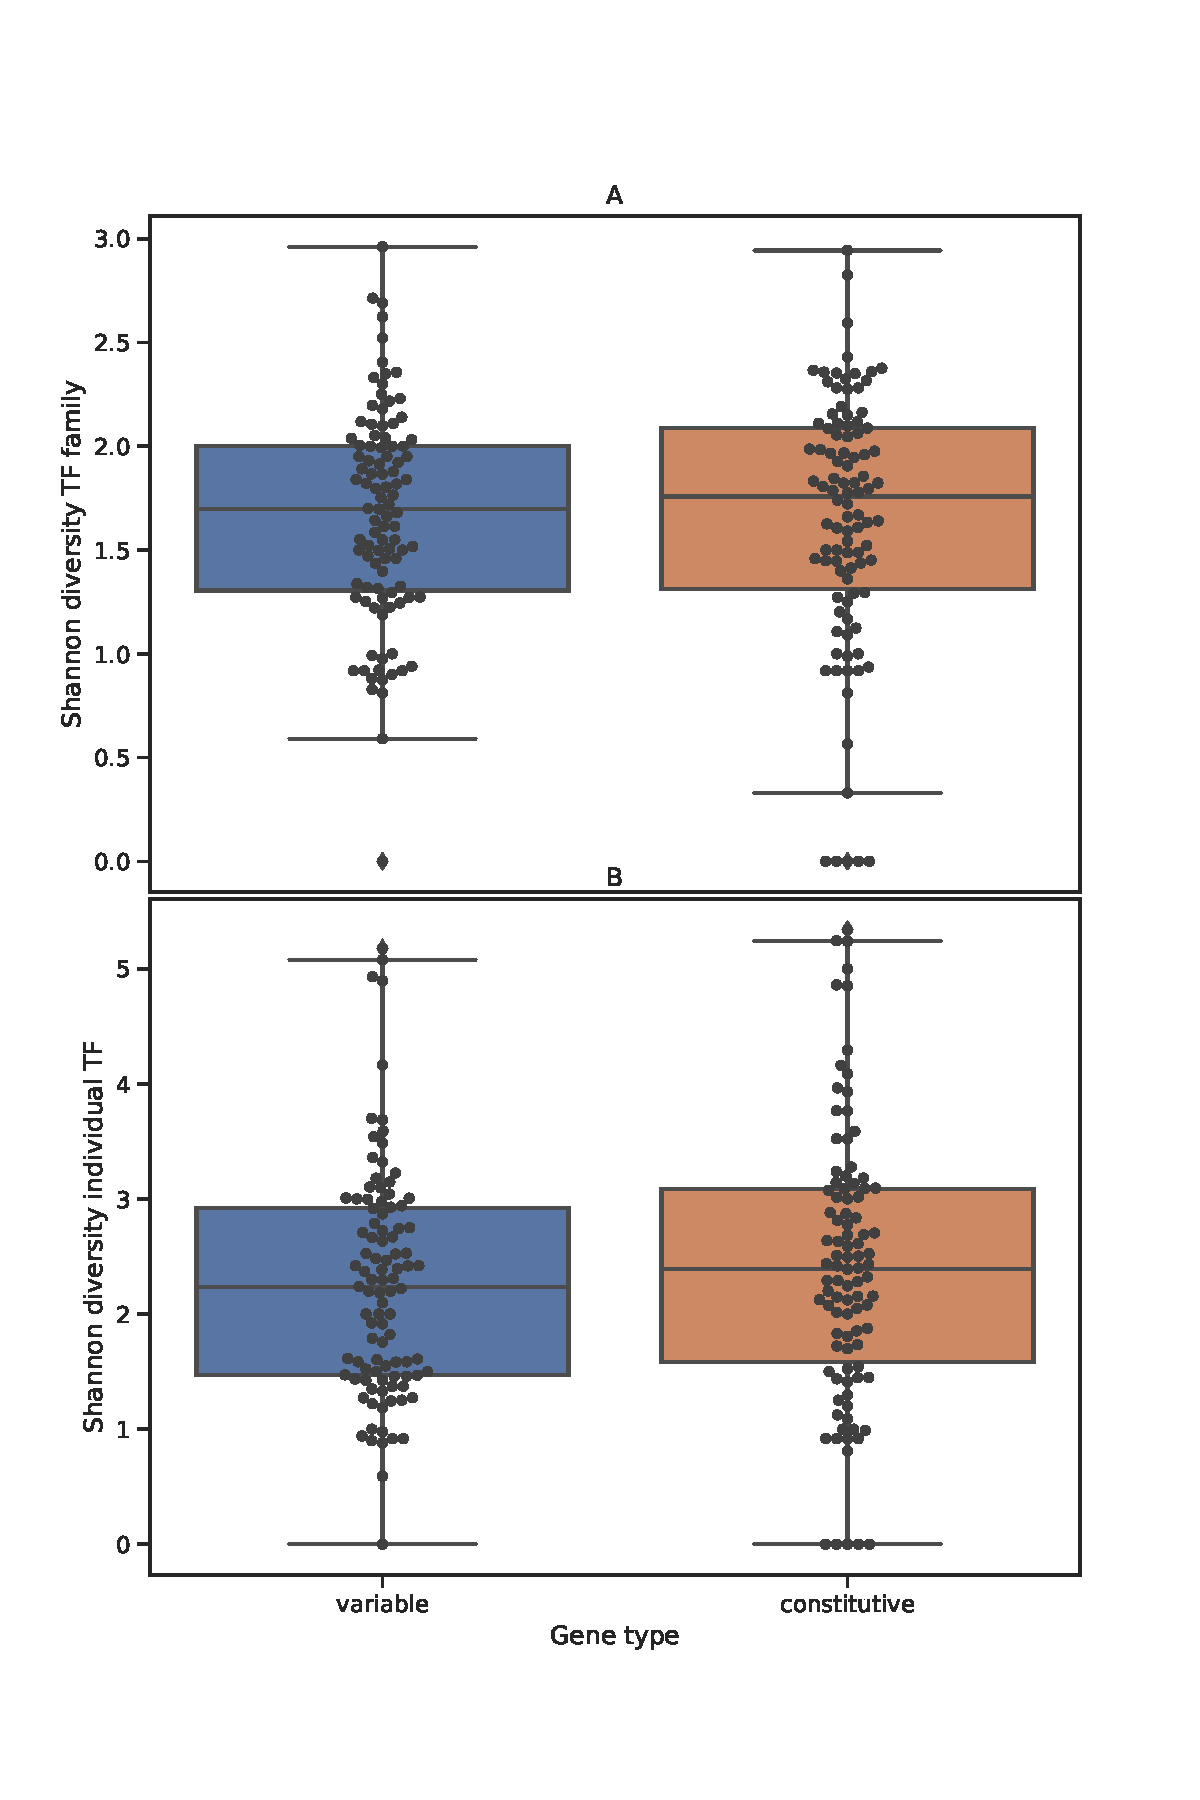
\includegraphics[width=0.70\columnwidth]{responsiveTF_diversity/responsive_histogram}
\caption{Shannon diversity of TF families (A) and individual TFs (B) binding the promoters of 100 variable (blue) and 100 constitutively expressed (orange) genes in \textit{A. thaliana}. Promoters were 1000 bp upstream of the annotated Araport 11~\autocite{chengAraport11CompleteReannotation2017} TSS.
\label{fig:diversity-histogram}
}
\end{center}
\end{figure}


To test the hypothesis that constitutive genes are bound by a different set of TF families than variable genes, Kmeans clustering was conducted. Kmeans clustering of the diversity of TF families binding a promoter did not correspond to gene type (\autoref{fig:pca}).
Unique TFBS counts (Mann\hyp{}Whitney~\textit{U} = 4680,~\textit{p} \textgreater{} 0.05)
and raw TFBS counts (Mann\hyp{}Whitney~\textit{U} = 4660,~\textit{P}
\textgreater{} 0.05) within promoters also did not differ significantly between promoter types.

\begin{figure}[!ht]
	\begin{center}
		\capstart
		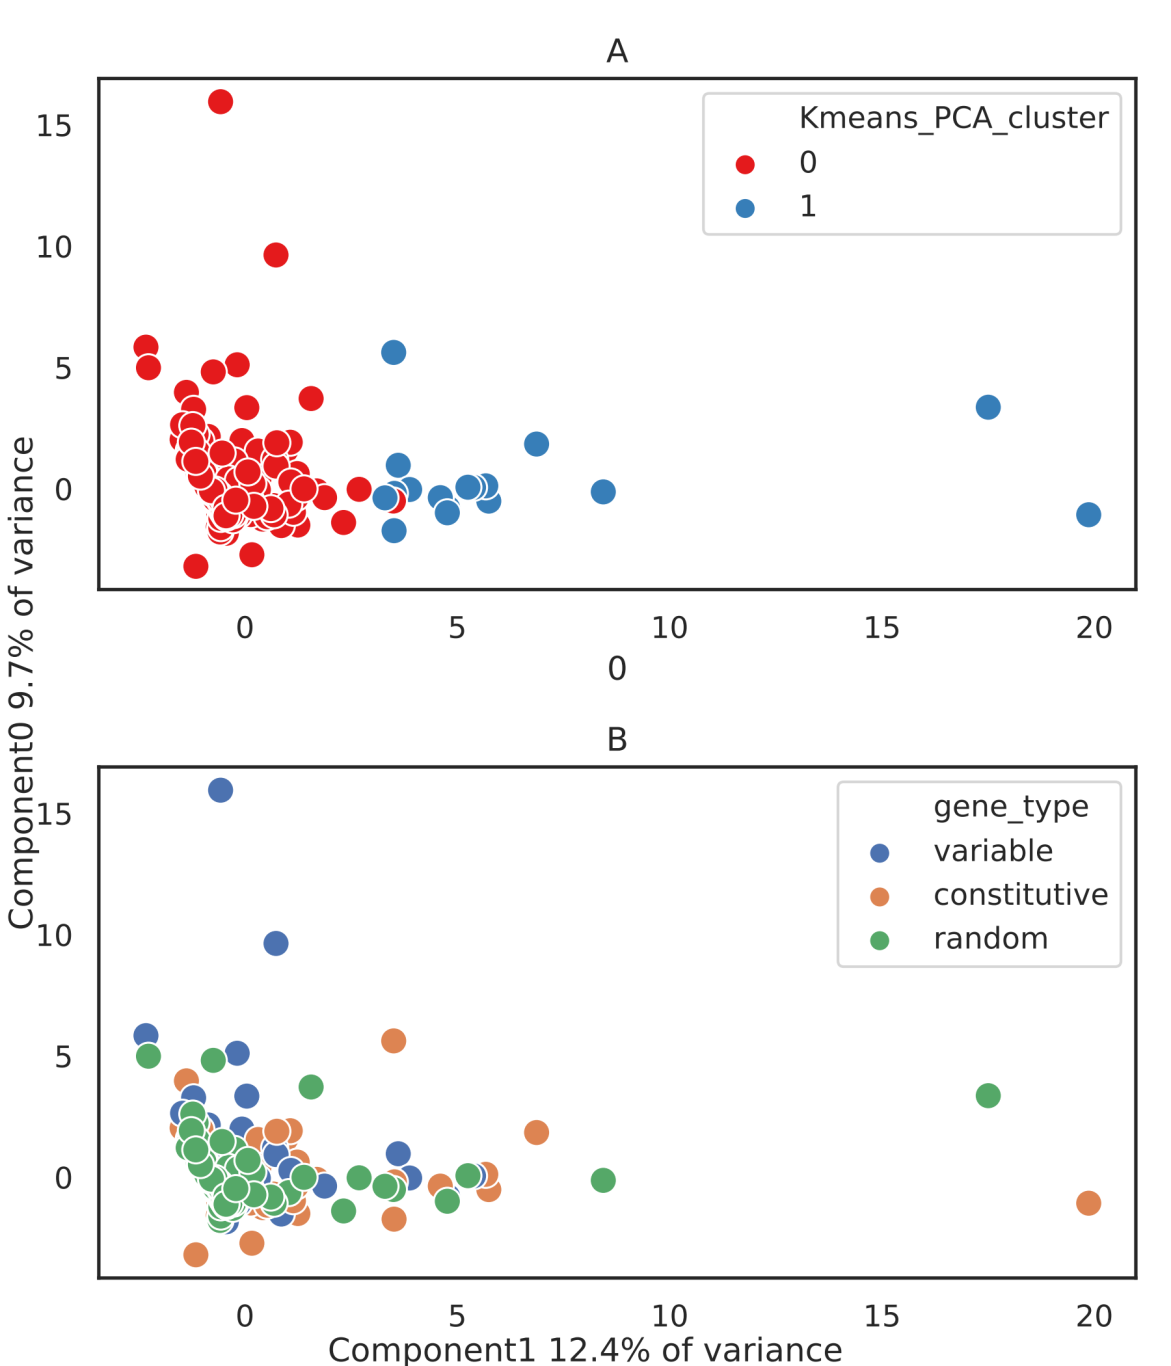
\includegraphics[width=0.70\columnwidth]{responsiveTF_diversity/responsiveTF_diversity_kmeans}
		\caption{Two PCA components accounting for the highest \si{\percent} of variation for Shannon diversity of TF families binding promoters. A, points coloured with two Kmeans clusters. B, points coloured by gene type. Variable genes, blue. Constitutive genes, orange. Random genes (across a range of coefficient of variation values), green.
			\label{fig:pca}
		}
	\end{center}
\end{figure}

\subsection{Results: TATA box enrichment}
Enrichment of 15 bp TATA boxes was compared between constitutive and
variable genes to test the hypothesis that variable genes are enriched in TATA boxes. Variable gene promoters were enriched in TATA boxes (total TATA boxes = 26; observed bp=390; expected bp=195; log2fold=0.52;~\textit{P} \textless{} 0.01) compared to the background of all 200 constitutive and responsive promoters
(\autoref{fig:enrichment}). Conversely, constitutive gene
promoters had significantly fewer TATA boxes compared to the background of all 200 constitutive and variable promoters (total TATA boxes = 11; observed bp=164; expected bp=1281; log2fold=-0.77;~\textit{P} \textless{} 0.01).

\begin{figure}[!h]
\begin{center}
\capstart
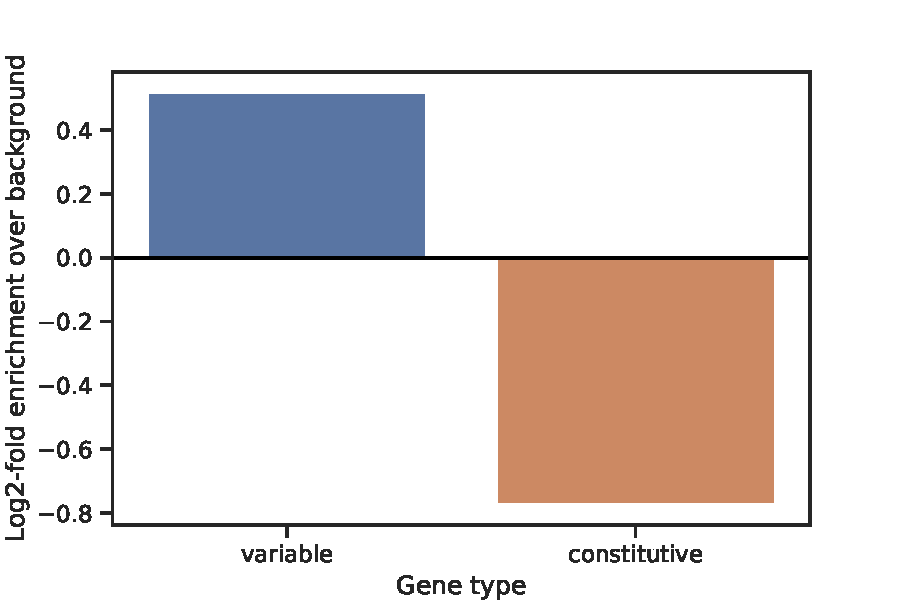
\includegraphics[width=0.70\columnwidth]{log2fold/log2fold}
\caption{Log2\hyp{}fold enrichment of 15 bp TATA boxes in variable (blue) and constitutive (orange) gene promoters compared to a background of
constitutive and variable promoters combined.~\textit{N~}= 100. Promoters were 1000 bp upstream of the Araport 11 \autocite{chengAraport11CompleteReannotation2017} annotated
transcription start site and included 675 bp downstream too. TATA box
locations downloaded from Eukaryotic Promoter Database
\autocite{dreosInfluenceRotationalNucleosome2016}. Gat software~\autocite{hegerGATSimulationFramework2013} was used to calculate enrichment.
\label{fig:enrichment}
}
\end{center}
\end{figure}

\subsection{Results: Labwork}
52 level 1 plasmids were constructed (supplementary table 1). These
include the 24 constitutive\fshyp{}N\hyp{}responsive promoters of 500 bp and 1000 bp size, controlling the nano luciferase gene, the various positive and negative controls and also the \textit{E. coli} and cell free protein expression plasmids. Previous experiments showed that root biomass from plants grown on vertical plates was not high enough for protoplast extraction. To increase root biomass Arabidopsis was grown using hydroponics. Hydroponics plants in nitrate free medium were very small (\autoref{fig:hydroponics-photo}) so a batch containing glutamine
too was grown. These plants were also very small with not enough root
biomass for protoplast experiments so it was decided that all plants
would be grown in replete medium and then be transferred to depleted
medium for three days.
\begin{figure}[!h]
\begin{center}
\capstart
\includegraphics[width=0.70\columnwidth]{figure/figure}
\caption{
5, 4 and 3 week old \textit{Arabidopsis thaliana} hydroponics plants grown in nitrate free 1/4 Hoaglands medium (A) and replete nitrate 1/4 Hoaglands medium (B). Since plants were so small in nitrate free medium it was decided that all plants would be grown in replete medium until large enough and then depleted from nitrate later on.
\label{fig:hydroponics-photo}
}
\end{center}
\end{figure}

Root protoplast luminescence was also low and close to the background
levels. It was hypothesised that leaf protoplast transient expression is high because they are left in the light to photosynthesise overnight. As root protoplasts are unable to photosynthesise, they were resuspended in K3G1 growth medium overnight instead of W5 solution. In a preliminary
experiment this increased luminescence
(\autoref{fig:root-solution-luminescence}). However, due to a sample size of 1 for the W5 condition no statistical analyses were performed on this data.

\begin{figure}[!h]
\begin{center}
\capstart
\includegraphics[width=0.70\columnwidth]{promoter_luminescence/promoter_luminescence}
\caption{
Mean luminescence of \textit{Arabidopsis thaliana} root protoplasts in W5 solution (orange bars) vs K3G1 nutrient solution (blue bars). \SI{20}{\micro\gram} of
LucN expressing plasmids and \SI{10}{\micro\gram} of delivery calibrator
(\textit{35S}:LucF and \textit{UBQ10}:LucF) plasmids were used during
transformation. \textit{STAP4}, negative control. Plant tissue was from 3-6 week old hydroponically grown plants. Error bars, \SI{68}{\percent} confidence intervals (1 Standard error). K3G1 \textit{n} = 2. W5 \textit{n} = 1.
\label{fig:root-solution-luminescence}
}
\end{center}
\end{figure}

Expression of \textit{UBQ10}, \textit{NIR1}, \textit{NOS}, \textit{STAP4}, \textit{NRP} promoters did not differ significantly under different nitrate treatments~in Arabidopsis leaf protoplasts (Kruskal\hyp{}Wallis, \textit{p} \textgreater{} 0.05) (\autoref{fig:leaf-nitrate-depletion}).

\begin{figure}[!h]
\begin{center}
\capstart
\includegraphics[width=0.70\columnwidth]{promoter_luminescence_corrected/promoter_luminescence}
\caption{
Mean luminescence of various promoters expressing in \textit{Arabidopsis thaliana} leaf protoplasts in different conditions with and without nitrate. The experiment calibrator for all promoters was \textit{UBQ10}:LucF. Protoplasts extracted from 8 week old hydoponically grown plants. Plants were transferred to nitrate depleted medium 4 days before protoplast extraction. Nitrate responsive promoters, \textit{NIR1}
and \textit{NRP}. \textit{NRP}\_NLP7\_TF was a co\hyp{}expression of \textit{NRP} and the NLP7 transcription factor which was only done under W5 nitrate free conditions. \textit{N} = 3. Error bars, \SI{68}{\percent} confidence intervals (1 standard error).
\label{fig:leaf-nitrate-depletion}
}
\end{center}
\end{figure}

Various promoters were tested in leaf protoplasts extracted from plants grown on nitrate free medium hydroponics, with and without \SI{10}{\milli\Molar} nitrate added to the protoplasts two hours before taking a reading. None of the promoters responded significantly to nitrate
(\autoref{fig:leaf-nitrate-constant}).
\begin{figure}[!ht]
\begin{center}
\capstart
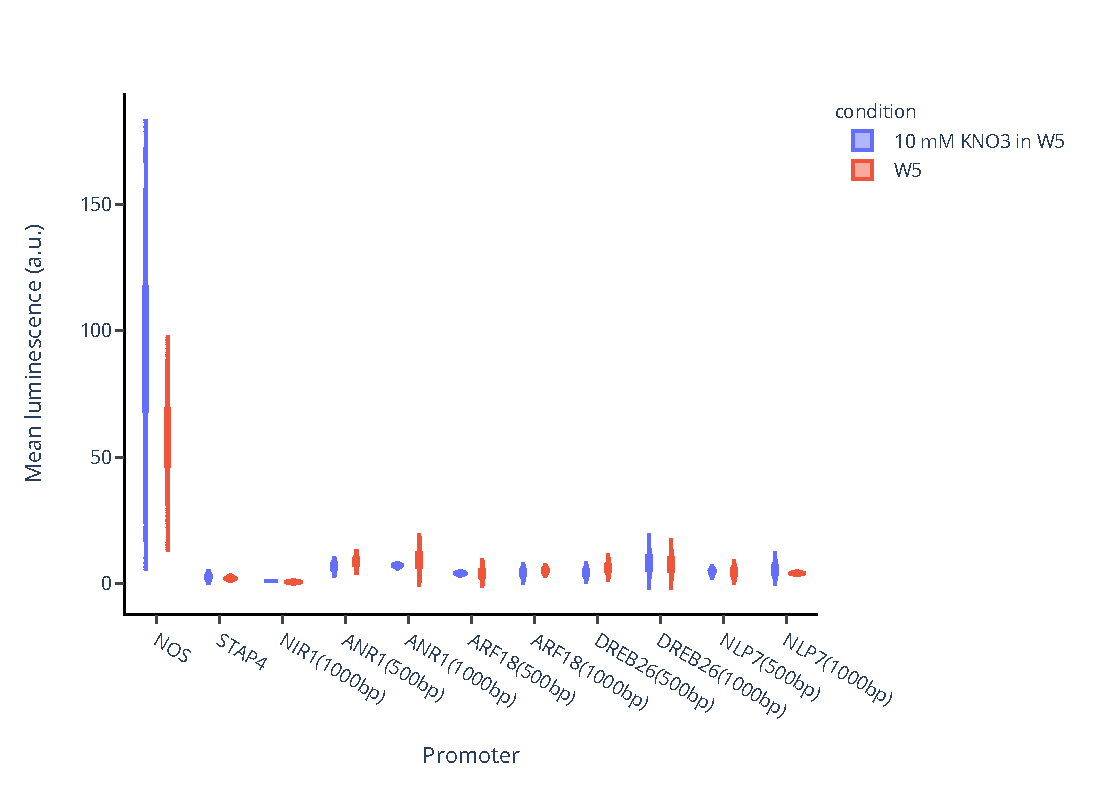
\includegraphics[width=1.00\columnwidth]{24-9-19/violin23.9.19}
\caption{
Mean luminescence of various promoters expressing in~\textit{Arabidopsis
thaliana~}leaf protoplasts in different conditions with and without
nitrate. Plants were grown in nitrate\hyp{}free hydroponics medium.
Protoplasts were extracted and left in W5 solution overnight, and then
either \SI{10}{\milli\Molar} KNO\textsubscript{3} in W5 solution (blue) or W5 solution
(red) was added. Plot is a violin plot showing a rotated kernal density
on each side and also a box\hyp{}plot.
\label{fig:leaf-nitrate-constant}
}
\end{center}
\end{figure}



Promoters were co\hyp{}expressed with TFs transiently in leaf protoplasts (\autoref{fig:co-expression}). Promoter \textit{NIR1} combinations were found to differ significantly using a Kruskal-Wallis test ($\chi^2$(5) = 20.82;~\textit{P} \textless{} 0.001).
%reference tests!
Dunn's posthoc tests showed that the \textit{NIR1} promoter luminescence was significantly increased when co\hyp{}expressed with NLP7 (22.5 ± 10.5 luminescence;~\textit{P} \textless{} 0.05), a combination of NLP6 and NLP7 (30.7 ± 14.6 luminescence;~\textit{P} \textless{} 0.01) compared to when it was co\hyp{}expressed with the DREB26 TF (0.8 ± 0.2 luminescence).
Promoter \textit{ANR1} combinations were found to differ significantly using a Kruskal-Wallis test ($\chi^2$(4) = 14.88;~\textit{P} \textless{} 0.01).
Dunn's post-hoc tests revealed that the \textit{ANR1} promoter luminescence was significantly higher when co\hyp{}expressed with DREB26 (8.1 ± 8.6 luminescence) than when it was co\hyp{}expressed with the ANR1 TF (2.0 ± 0.7 luminescence; \textit{P} \textless{} 0.01) or NLP7 (1.4 ± 0.6 luminescence; \textit{P} \textless{} 0.001).
The \textit{ANR1} promoter luminescence was significantly higher when co\hyp{}expressed with ARF18 (2.7 ± 1.0 luminescence) than when it was co\hyp{}expressed with NLP7 (1.4 ± 0.6 luminescence; \textit{P} \textless{} 0.05).

\begin{figure}[!h]
\begin{center}
\capstart
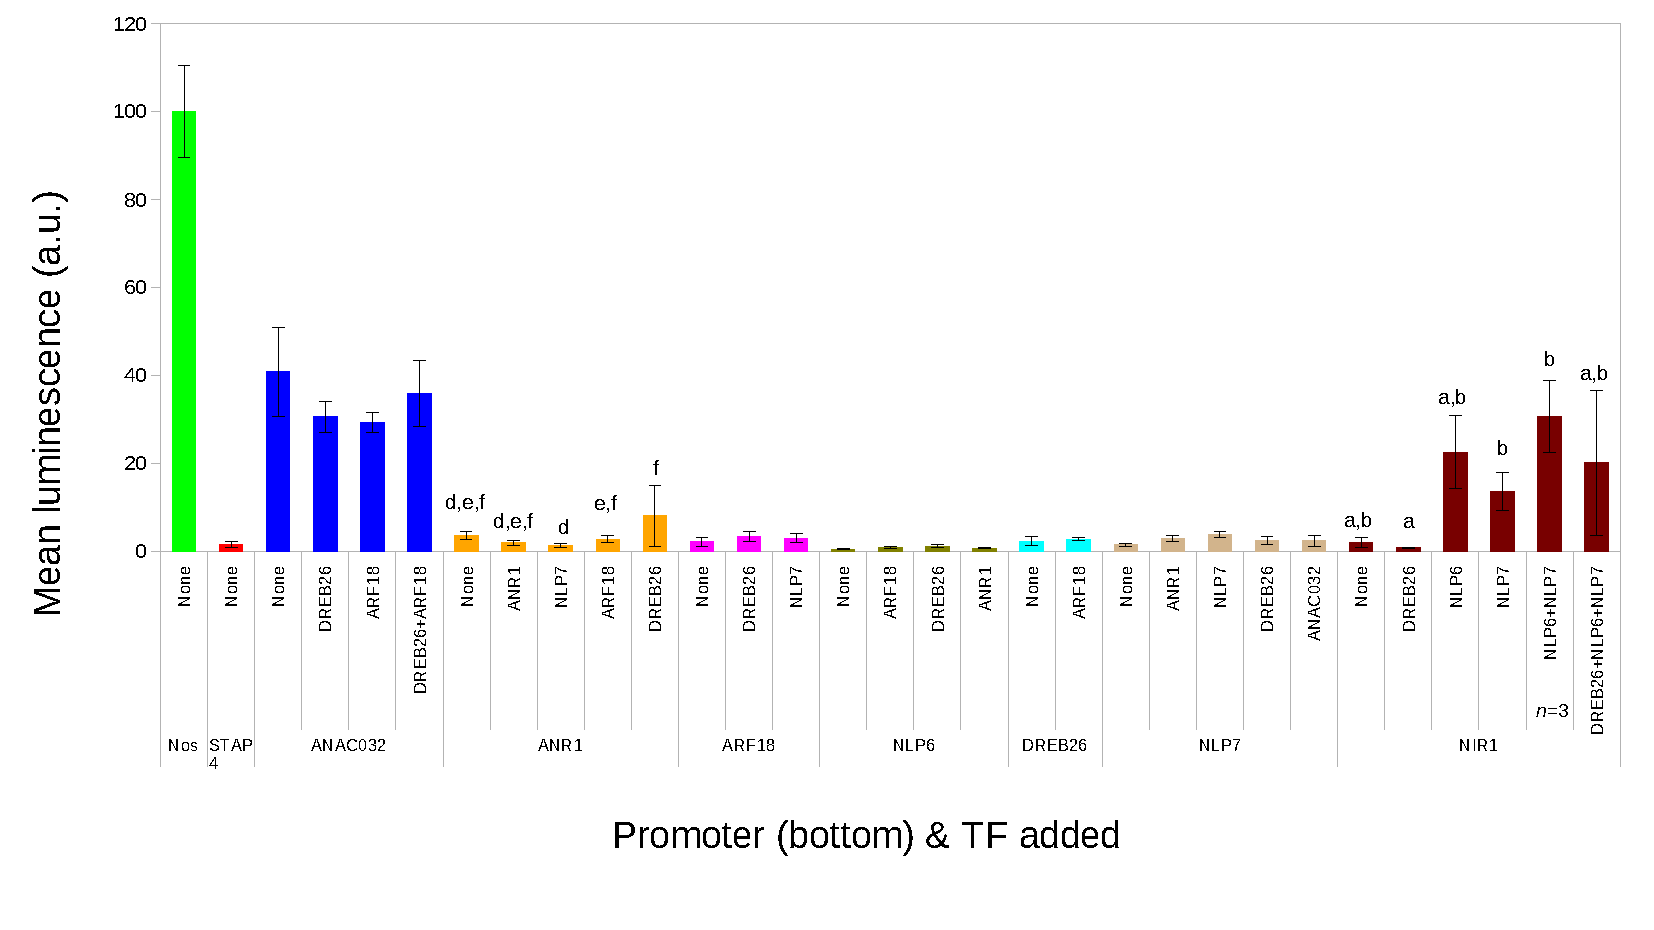
\includegraphics[width=1.00\columnwidth]{TF_coexpression_visualisationtest/TF_coexpression_visualisation}
\caption{
Mean luminescence of various transiently expressed promoters with or without co\hyp{}expressed transcription factors predicted to bind them in \textit{Arabidopsis thaliana} leaf protoplasts.
On the x\hyp{}axis promoter names are horizontal at the bottom, co\hyp{}expressed TF names vertical. Different letters above bars of the \textit{NIR1} and \textit{ANR1} promoters represent statistically significant differences, according to Kruskal-Wallis followed by Dunn's post-hoc tests with bonferonni multiple correction (\textit{P} \textless{} 0.05). The expression of the different promoters were not compared to each other.
Plants were grown in hydroponics 1/4 Hoagland replete nitrate medium for 6 weeks.
\textit{n} = 6\hyp{}12 apart from the \textit{NIR1} promoter co\hyp{}expressed with NLP6+NLP7 TFs where~\textit{n} = 3.
Error bars, \SI{95}{\percent} confidence intervals.
\label{fig:co-expression}
}
\end{center}
\end{figure}

\section{Discussion}{\label{discussion}}

Various hypotheses were tested with the bioinformatics pipeline. The hypothesis that the percentage coverage of TFBSs in promoters is higher in constitutively expressed genes than in variable was not accepted as percentage coverage did not differ significantly between promoter types.
Likewise, the hypothesis that  GC content is higher in constitutive genes than in variable genes was also not accepted as GC content did not vary significantly between promoter types. 
The Shannon diversity of TFs and TF families binding promoters did not differ significantly so the hypothesis that constitutive genes would be bound by more diverse TFs and TF families than variable genes was not accepted.
Similarly, raw and unique TFBS counts did not differ significantly between constitutive and responsive promoters.
However, many of the promoters tested were overlapping other genes (122/200) and 80/200 of the promoters tested had an upstream gene oriented in the opposite direction within 2000 bp of the TSS so they could potentially be sharing promoters.
In future analyses it will be important to filter out these overlapping genes or at least reduce the promoter length so they are no longer overlapping as it is hard to determine which features belong to which gene when they are overlapping.
\textcite*{mattioliHighthroughputFunctionalAnalysis2019} found that promoters in three human cell lines with highly overlapping TFBSs were associated with high
expression and low specificity so were more ubiquitously expressed.
Promoters that had lower, more specific expression had fewer overlapping TFBSs. This does not seem to apply to Arabidopsis where there was no significant difference between Shannon diversity of TFs and TF families binding constitutive or responsive promoters, and there was also no obvious clustering of TF families between constitutive and responsive promoters (\autoref{fig:pca}).
In \textcite*{czechowskiGenomeWideIdentificationTesting2005} the top most constitutively expressed genes were also in the top \SI{20}{\percent} lowest expressed genes. 
This also contradicts \textcite*{mattioliHighthroughputFunctionalAnalysis2019}, where constitutive promoters were more strongly expressed.
\textcite*{mattioliHighthroughputFunctionalAnalysis2019} also found that constitutive promoters had more bps covered by TFBSs than tissue\hyp{}specific promoters, which contradicts the finding in Arabidopsis where there was no significant difference (\autoref{fig:bp-covered}).

In insects~\autocite{engstromGenomicRegulatoryBlocks2007} and mammals~\autocite{carninciGenomewideAnalysisMammalian2006} TATA boxes are enriched in variably expressed genes compared to constitutively expressed genes. This was hypothesised to be true in Arabidopsis so was tested in the bioinformatics pipeline. Arabidopsis variable genes were significantly enriched for TATA boxes compared to constitutive genes (\autoref{fig:enrichment}), proving the hypothesis correct.
When promoters were designed to increase expression using machine learning, variably expressed promoters already containing a TATA box were given additional TA repeat sequences at the 5' end of the 246 bp promoter and these increased expression.
Promoters with longer TATA boxes had higher expression~\autocite{kotopkaModeldrivenGenerationArtificial2020}.
In the same study they also predicted and tested constitutive promoters with increased expression.
The constitutive promoters predicted and tested to have higher expression contained more TFBSs throughout the promoter from 7 different groups.
These promoters were not enriched for TA repeat sequences, suggesting that TA repeat sequences are more important in variably expressed promoters.
This further backs up the results that variable genes are enriched for TATA boxes.
In mouse and human promoters TATA boxes were strongly over\hyp{}represented in promoters showing sharp TSSs, whereas CpG island were associated with broad TSS regions~\autocite{carninciGenomewideAnalysisMammalian2006}.
In Arabidopsis, there is an association of TATA boxes with narrow TSS peaks, and GA elements with broader TSS peaks~\autocite{yamamotoHeterogeneityArabidopsisCore2009}.
In a later study a higher percentage of TATA boxes were found in narrow TSS peak promoters than broad or weak peak promoters but they found no significant difference when a more stringent control of false positive TATA boxes was used~\autocite{mortonPairedEndAnalysisTranscription2014}.
In human promoters, CpG elements are associated with constitutive genes~\autocite{schugPromoterFeaturesRelated2005,saxonovGenomewideAnalysisCpG2006} whereas Arabidopsis GA\hyp{}type promoters showed no such association~\autocite{yamamotoHeterogeneityArabidopsisCore2009}.
In \textcite*{mortonPairedEndAnalysisTranscription2014} narrow peak promoters were associated with strongly expressed, variable genes, while weak TSS peak promoters were associated with constitutive genes with lower expression.
Broad peak promoters had qualities of both narrow and weak TSS peak promoters and were associated with processes with strong gene expression routinely at certain times in the circadian cycle.
This suggests that variable genes are enriched for TATA boxes, are highly expressed and have a narrow TSS peak, while constitutively expressed genes tend not to have TATA boxes, have a weak TSS peak and have lower gene expression.

It was hypothesised that root protoplasts would need growth medium to increase protein expression as unlike leaf protoplast they cannot photosynthesise. This was tested in a preliminary experiment and indeed the addition K3G1 growth medium increased luminescence in root protoplasts (\autoref{fig:root-solution-luminescence}), although this needs to repeated with more samples for analysis.

It was expected that \textit{NIR1} and \textit{NRP} would respond to nitrate as they have in previous studies \autocite{liuDiscoveryNitrateCPKNLPSignalling2017, wangMultipleRegulatoryElements2010}. 
Transient expression of \textit{UBQ10}, \textit{NIR1}, \textit{NOS}, \textit{STAP4}, \textit{NRP} promoters did not differ significantly under different nitrate treatments in Arabidopsis leaf protoplasts
(\autoref{fig:leaf-nitrate-depletion}).
However, the experimental calibrator \textit{UBQ10}:LucF did seem to differ between nitrate treatments which could be hiding the response of the other promoters as these were normalised to \textit{UBQ10}:LucF.
\textit{UBQ10} is a constitutively expressed promoter~\autocite{czechowskiGenomeWideIdentificationTesting2005} and is used as a calibrator in many nitrate studies \autocite{konishiArabidopsisNINlikeTranscription2013a,liuDiscoveryNitrateCPKNLPSignalling2017,satoDirectTranscriptionalActivation2017} so the reason for its response to different nitrate conditions is uncertain and needs to be investigated.
It could be that in the nitrate free condition the cell metabolisms had slowed, and when nitrate was added the metabolism increased again.
The results in \autoref{fig:leaf-nitrate-depletion} contradict a study where Arabidopsis was grown on nitrate free agar and when \SI{10}{\milli\Molar} KNO\textsubscript{3} was added for 2 hours to seedlings or extracted leaf protoplasts, \textit{NIR1} was induced \textasciitilde{}18\hyp{}fold and \textasciitilde{}12\hyp{}fold respectively compared to the addition of \SI{10}{\milli\Molar} KCl \autocite{liuDiscoveryNitrateCPKNLPSignalling2017}.
\textit{NRP} is known to be induced 5.9\hyp{}fold in response to nitrate
too \autocite{wangMultipleRegulatoryElements2010}.
To see how \textit{NIR1} and \textit{UBQ10} in a genomic context respond to the nitrate conditions samples were frozen in liquid nitrogen and then stored at \SI{-70}{\degreeCelsius} for future RNA extraction and analysis with qRT\hyp{}PCR.
\textcite*{konishiIdentificationNitrateresponsiveCiselement2010a} found that the native Arabidopsis \textit{NIR1} gene expression increased \textasciitilde{}20\hyp{}fold after the addition of \SI{10}{\milli\Molar} KNO\textsubscript{3} compared to \SI{10}{\milli\Molar} KCl.
In this study seedlings were grown in nitrogen\hyp{}free liquid medium for 3.5 days before the addition of nitrate.

In leaf protoplast co\hyp{}expression analyses~\textit{NIR1} expression was induced by NLP7, NLP6 + NLP7 and seemed to be repressed by DREB26 (\autoref{fig:co-expression}).
The \textit{NIR1} promoter has the known 43 bp nitrate\hyp{}responsive \textit{cis}\hyp{}element (NRE) binding site for NLP7 and NLP6 transcription factors so this was as expected~\autocite{konishiArabidopsisNINlikeTranscription2013a}.
NLP7 is known to be actively pumped out of the nucleus under nitrate starvation and accumulates in the nucleus through Ca\textsuperscript{2+} binding in response to nitrate by nuclear retention, where it induces nitrate\hyp{}regulated genes such as \textit{NIR1}~\autocite{marchiveNuclearRetentionTranscription2013b}.
The other promoters \textit{ANAC032}, \textit{ANR1}, \textit{ARF18}, \textit{NLP6}, \textit{DREB26} and \textit{NLP7} did not respond significantly to the co\hyp{}expressed TFs, suggesting that either the promoters were not direct targets of the co\hyp{}expressed TFs, or that they required other cofactors to be activated. The fact that the \textit{NIR1} promoter used in protoplast experiments responded to NLP7 but not to nitrate suggests that the nitrate response pathway mediated by NLP7 was not activating under the experimental conditions used. As shown in \autoref{fig:leaf-nitrate-depletion}, \textit{NRP} co\hyp{}expressed with NLP7 looked to be expressed higher than \textit{NRP} with and without nitrate, again suggesting the NLP7 was not responding as expected in the nitrate response pathway. Alternatively it could be that \textit{NIR1} and \textit{NRP} do respond to nitrate but the response is quick and then expression returns to basal levels afterwards all within the two hours. Indeed, NLP7 nuclear localisation by phosphorylation occurs within minutes of N supply~\autocite{marchiveNuclearRetentionTranscription2013b,liuDiscoveryNitrateCPKNLPSignalling2017}. NLP7 binding to its genome\hyp{}wide targets was highest 5 minutes after nuclear import~\autocite{alvarezTransientGenomewideInteractions2020}.
In the same co\hyp{}expression analysis \textit{ANR1} expression was induced higher when co\hyp{}expressed with DREB26 than with the ANR1 or NLP7 TFs. \textit{ANR1} expression was higher when it was co\hyp{}expressed with ARF18 than with NLP7. NLP7 seemed to repress expression of \textit{ANR1} while DREB26 looked to increase expression. A yeast\hyp{} hybrid assay both DREB26 and ARF18 were shown to bind the \textit{ANR1} promoter~\autocite{gaudinierTranscriptionalRegulationNitrogenassociated2018}. NLP7 did not bind the \textit{ARF18} promoter in a TARGET assay~\autocite{alvarezTransientGenomewideInteractions2020} or in the yeast\hyp{}one hybrid assay~\autocite{gaudinierTranscriptionalRegulationNitrogenassociated2018}. Therefore the repression effect of NLP7 is could be due to an indirect effect where NLP7 regulates a different TF and then that regulates \textit{ANR1}.

\section{Future work}
{\label{future-work}}

Include gantt chart

In chapter one the promoters being used for analyses will be expanded to include the 5'UTR to ensure that all of the possible TSSs and any surrounding TFBSs are included.
The promoters will also be shortened to exclude parts that overlap other genes as evolutionary contraints on coding genes are more stringent than non\hyp{}coding regions.
Therefore, overlapping genes might hide the general logic of the non\hyp{}coding regions.
Since more constitutive genes (53) than variable genes (27) were flagged as having potentially overlapping promoters, a comparison between constitutive and variable genes will be done to investigate whether more constitutive genes than variable genes putatively share a promoter with upstream genes facing the opposite direction.
Promoters head\hyp{}to\hyp{}head on opposite strands within 2000 bp will be classed as divergent.
Bidirectional promoters are underrepresented for TATA boxes~\autocite{dhadiGenomewideComparativeAnalysis2009}.
Since variable genes are enriched for TATA boxes, this suggests that constitutive promoters lacking TATA boxes are be more likely to be bidirectional.
This hypothesis will be tested in the future.
In humans, GA\hyp{}repeat regions were associated with divergent promoters. Additionally, the introduction of a GA\hyp{}binding protein binding site into unidirectional promoters turned \SI{67}{\percent} of them into bidirectional promoters~\autocite{collinsEtsRelatedTranscriptionFactor2007}.
This suggests that certain TFBSs can change directionality.
Since variable promoters are depleted in GA\hyp{}repeat regions~\autocite{yamamotoHeterogeneityArabidopsisCore2009}, a hypothesis would be that constitutive promoters are more likely to be divergent and bidirectional.
However, in humans GA\hyp{}repeat regions are bound by the ETS\hyp{}family GA\hyp{}binding protein~\autocite{collinsEtsRelatedTranscriptionFactor2007} whereas in plants by the BARLEY B RECOMBINANT / BASIC PENTACYSTEINE (BBR/BPC) family~\autocite{theunePhylogeneticAnalysesGAGAMotif2019}, so they may function differently.
Since no correlation was found for TF and TF family diversity and also for TFBS percentage coverage between 1000 bp constitutively and variably expressed promoters, a higher emphasis will be applied to TFBSs within 100 bp from the TSS as motifs throughout human~\autocite{fitzgeraldClusteringDNASequences2004} and \textit{Drosophila}~\autocite{fitzgeraldComparativeGenomicsDrosophila2006} promoters only corresponded to biological function within the 100 bp region.

Although the coding sequences (CDSs) of mammalian constitutive genes evolve more slowly than those of variable genes~\autocite{zhangMammalianHousekeepingGenes2004}, the promoters of constitutive genes were less conserved than in variable genes \autocite{farreHousekeepingGenesTend2007}.
However, in pigs both promoters and CDSs of constitutive genes were more conserved than those of variable genes~\autocite{weiCharacterizationGenePromoters2019}.
These contradictions suggest that complexity of regulation in GRNs is lost when just comparing constitutive to variable genes, and comparisons need to include more information about the regulatory context.
Genes coding for master-regulator TFs are classed as multi\hyp{}interface (MI) hub genes, while those coding for lesser connected TFs are classed as single interface (SI) hub genes.
Within MI genes, constitutive and variable CDSs showed similar evolution rates, while within SI genes constitutive gene CDSs evolve more slowly than variable gene CDSs~\autocite{podderMultifunctionalityDominantlyDetermines2009}.
MI variably expressed genes evolved more slowly than SI variably expressed genes, while both MI and SI constitutively expressed genes evolved at similar rates~\autocite{biswasEvolutionaryRateHeterogeneity2018}.
This was explained by the fact that variable MI genes are bound by more miRNAs than variable SI genes~\autocite{biswasEvolutionaryRateHeterogeneity2018}, and genes with more miRNA targets evolve more slowly ~\autocite{chengRelationshipEvolutionMicroRNA2009}.
DNA entropy is a proxy for how many random sequence patterns there are, with a lower entropy meaning more non-random DNA features.
In humans, variable gene promoters have a lower DNA entropy than those of constitutive genes, suggesting that variable gene promoters have a higher density of TFBSs than constitutive genes~\autocite{thomasDNAEntropyReveals2015}.
The density of motifs in variable promoters is higher than in constitutive promoters in pigs~\autocite{weiCharacterizationGenePromoters2019}, further backing up that variable promoters containg more TFBSs.
However, this is contradicted by \textcite{mattioliHighthroughputFunctionalAnalysis2019} where constitutive promoters contained a higher density of TFBSs.
A hypothesis to test in plants would be that the CRE landscapes of constitutive genes will be more complex than in variable genes and so will be relatively less conserved than variably expressed genes.

In plants, highly expressed gene CDSs are often longer than genes with lower expression whereas the opposite is true for animals~\autocite{renPlantsHighlyExpressed2006}.
Highly expressed genes in \textit{S. cerevisiae}~\autocite{drummondWhyHighlyExpressed2005} and humans~\autocite{berthelotComplexityConservationRegulatory2018} evolve more slowly than genes with lower expression.
Since variable genes in plants tend to be more highly expressed than constitutive genes~\autocite{czechowskiGenomeWideIdentificationTesting2005, mortonPairedEndAnalysisTranscription2014}, they might also be longer.
This could be tested in Arabidopsis in the future.
However, in mammals constitutive genes have been reported as both longer~\autocite{zhuNatureHumanHousekeeping2008} and shorter~\autocite{eisenbergHumanHousekeepingGenes2003,weiCharacterizationGenePromoters2019} than variably expressed genes.

On the contrary to plants, constitutive genes in humans~\autocite{zhuNatureHumanHousekeeping2008,mattioliHighthroughputFunctionalAnalysis2019} and pigs~\autocite{weiCharacterizationGenePromoters2019} have higher expression than variable genes. 
~\textcite*{biswasEvolutionaryRateHeterogeneity2018} further showed that MI variable genes were more highly expressed than SI variable genes whereas there was no significant difference in expression level between MI and SI constitutive genes. In the future constitutive and variable genes could be split into MI and SI in Arabidopsis and further analysed.

It will also be important to incorporate chromatin accessibility into the bioinformatics pipeline to define promoter regions and also to compare constitutive and variable promoters as chromatin accessibility is expected to be maintained across different cell types in promoters of constitutive genes whereas accessbility will differ in variable genes depending on tissue or conditions.
Cell type\hyp{}enriched accessible regions (CTEARs) identified by ATAC-seq are associated with variable genes in both nematodes~\autocite{daughertyChromatinAccessibilityDynamics2017} and plants (Arabidopsis and tomato)~\autocite{kajalaInnovationConservationRepurposing2020b}.

In Arabidopsis, gene body methylation correlates with constitutive gene expression~\autocite{zhangGenomewideHighResolutionMapping2006, takunoBodyMethylatedGenesArabidopsis2012}, and methylation\hyp{}free gene bodies are associated with variable genes~\autocite{aceitunoRulesGeneExpression2008}. Unlike gene body methylation, promoter methylated genes show more variable gene expression~\autocite{zhangGenomewideHighResolutionMapping2006}. It will be important to factor in methylation data in future analyses.

Future work for the second thesis chapter will include checking for TF binding in promoters of nitrogen pathway master regulators using EMSA.
The qRT\hyp{}PCR analysis of endogenous \textit{NIR1} and \textit{UBQ10} response to nitrate in leaf protoplasts and leaves will also be completed to check they respond in the expected way to the conditions I apply to them.
Then the construction and delivery of a CRISPR library will be implemented to introduce genetic variation into regulatory regions of master\hyp{}regulators in the N\hyp{}responsive GRN.
This will involve identifying all possible CRISPR sites including those of the recent near PAM\hyp{}less Cas9~\autocite{waltonUnconstrainedGenomeTargeting2020}, followed by construction of sgRNAs and assembly of constructs containing Cas9\_sgRNA.
These will each be transferred into \textit{Agrobacterium tumefaciens}.
A liquid culture of all strains will be prepared and mixed to use for plant transformation.
Transgenic seeds (Arabidopsis T2) will be selected and then the target regions of many individuals will be sequenced to see which mutations they have accumulated. Progeny T2 seeds of lines with different mutations will be selected to assess phenotypes.

In the third thesis chapter genetic feedback will be engineered into the N\hyp{}responsive network.
Using a synthetic promoter created by Yaomin~\textit{et al}.~(unpublished) as a starting point, a synthetic promoter with the NRE binding sites for NLP6/NLP7 will be created and several versions with differing binding sites will be tested.
A dCas9\hyp{}activator and repressor which bind to the promoter of a N\hyp{}response master regulator that upregulates or represses expression will be built and tested.
These synthetic TFs will be controlled by the synthetic N\hyp{}responsive promoter and deployed as transgenes introducing positive or negative feedback.
Gene expression changes and phenotypes will be analysed to assess how the response to nitrate was changed.

\subsection{PIPs placement}
\label{pips-placement}

I recently embarked on my BBSRC Doctoral Training Partnership (DTP)
Professional Internships for PhD Students (PIPs) where I spent three
months working for Beneficial Bio. Beneficial Bio is a non\hyp{}profit
start\hyp{}up that uses a social franchise model to help establish
bioproduction labs in countries where resources are limited.
Social franchising is wheree commercial franchising concepts are used to promote social benefit rather than profit \autocite{beyelerImpactClinicalSocial2013}.
These labs produce low\hyp{}cost reagents and off\hyp{}patent enzymes to the local research community, improving accessibility of molecular biology.
The products sold by Beneficial Bio will not only be much cheaper than imports from the US, Europe and China, but are also more sustainable, have far faster delivery times and boost the local economy.
Beneficial Bio conducts its R\&D at the Biomakespace, a community lab in Cambridge, which is then implemented as a social franchise at MboaLab Biotech, a social enterprise in Cameroon.
The company is also in the process of setting up more production labs in other countries.

I spent the first two weeks of my placement in Cambridge, where I
prepared teaching material for my bioinformatics course, took photos of
products to put on the website and learnt low\hyp{}cost protein production
lab techniques. I then flew to Ghana and spent 2 months based at the
Kumasi Hive Hub, where the University of Cambridge's Open Bioeconomy Lab
recently funded a community biolab. My objectives in Ghana were to
conduct market research for Beneficial Bio and to contribute training based on the skills developed during my own research.
One of the courses I contributed to was a week\hyp{}long workshop teaching postgraduate and academic researchers the molecular biology techniques needed to
produce enzymes at a low\hyp{}cost. The enzyme they produced was a DNA
polymerase for use in PCR (polymerase chain reaction). Feedback from
participants was very positive, all indicating that they were much more
familiar with both theoretical and lab based techniques following the
course. A high number of participants also indicated that they would
like to teach the course, which will be run in more countries soon. The
plan is to release the content online for free alongside a low\hyp{}cost DIY
lab wiki explaining how to minimise lab costs and overcome problems.

I also ran a 4\hyp{}week bioinformatics training course that aimed to teach
students how to handle sequence data in command line Linux and Python \hyp{}
a course so high in demand that it was oversubscribed. The aim is to
have an autonomous bioinformatics club running to allow students to keep
practicing their skills. Running training courses for Beneficial Bio was
a great experience, it made me realise how much my skills have developed
during my PhD, and allowed me to impart that knowledge to students
without access to the high\hyp{}quality teaching resources available at
Earlham, making a real difference. Through running the teaching course I
have improved my organisational and planning skills along with
communication skills.

For the market research aspect of my placement, I travelled with my colleague
Harry Akligoh to the Volta region, where he showed me round his hometown
Keta, from where we journeyed on to Ho. Here we conducted market
research and interviewed several researchers at the University of Health
and Allied Sciences (UHAS) and the teaching hospital. I also conducted a
market research survey, from which we gained some very useful
information and hopefully will be the start of a future collaboration
with Beneficial Bio.

Another useful bit of experience I gained was in managing the Beneficial
Bio social media platforms, another important aspect of marketing and
brand awareness in the digital era. I was also able to advise on which
products Beneficial Bio should sell based on researcher needs, and
provided a financial projection recommending the prices of the products
after factoring in cost of production, overheads and studying the
competition. Through working for Beneficial Bio I gained an experience
of working for a startup company and greatly improved my commercial
awareness and business skills.

My placement has made me appreciate the good education I have had up
until now, and value the skills I have learnt. Being able to pass on the
things I've acquired was very rewarding, especially with the enthusiasm
and good feedback received from the participants.

I have learnt to be more independent and adaptable, thriving in a
country very different to the UK where things are much more spontaneous.
I have also gained experience in conducting market research in a market
very different to the UK, where consumers often have very different
factors influencing their decisions.